% \documentclass[12pt, oneside]{book}

\chapter{Surface gravity waves}
\label{chap:SurfaceWaves}
\begin{center}
    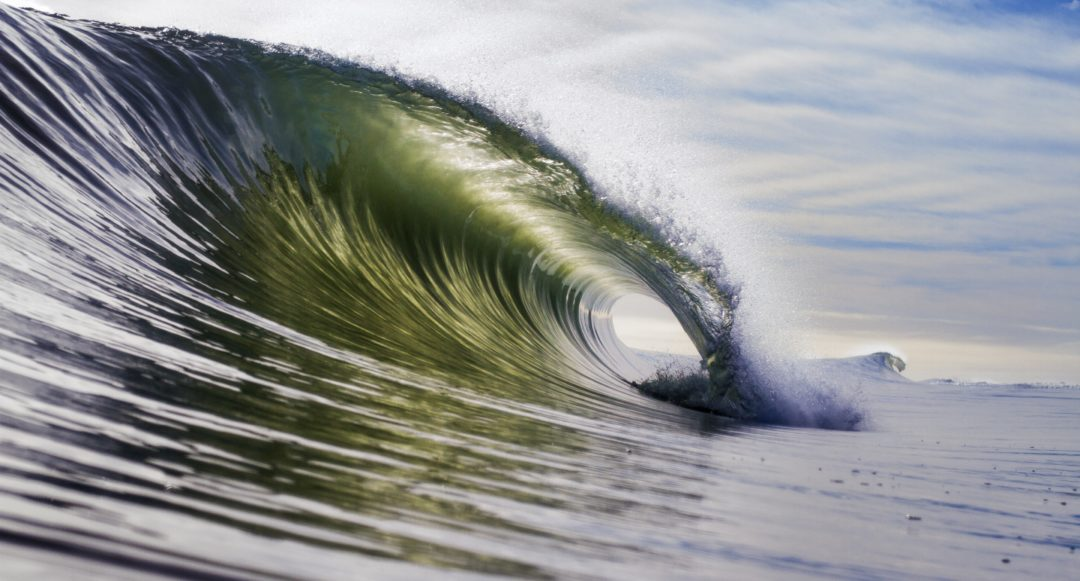
\includegraphics[width=6.5in]{BreakingWave.jpg}
\end{center}

Waves are the phenomena that carry energy from one place to another, and occur in all branches of physics, from sound waves, to the wave-like nature of light.   The ocean  supports waves, both at its surface, and on density interfaces within the ocean as touched on briefly in the previous part.  Here we deal just with surface waves though many of the same concepts apply to underwater waves and waves in the atmosphere.  We also restrict the discussion to high-frequency waves, and do not consider so-called ``planetary waves'' or waves that are strongly affected by rotation.  

\section{Characterizing waves}

Waves are often described in terms of sinusoids.  If we write out the equations that govern waves displacements the solutions are sinudoids, and indeed most waves we observer in nature are well approximated by sinusoids, \emph{except} near the shore, where non-linear effects can lead to breaking.  

So, if we took a photograph of a wave from the side, and froze it in time, the wave would be described by the height of the waves, or the \emph{amplitude}, $A$, and the distance between the wave crests (or troughs), or the \emph{wavelength}, $\lambda$.  The amplitude $A$ is usually the height of the wave crest from the resting interface of the water, and is half the crest-to-tough \emph{wave height} or $H$ \fref{fig:SketchDefnX}.  

\begin{marginfigure}
  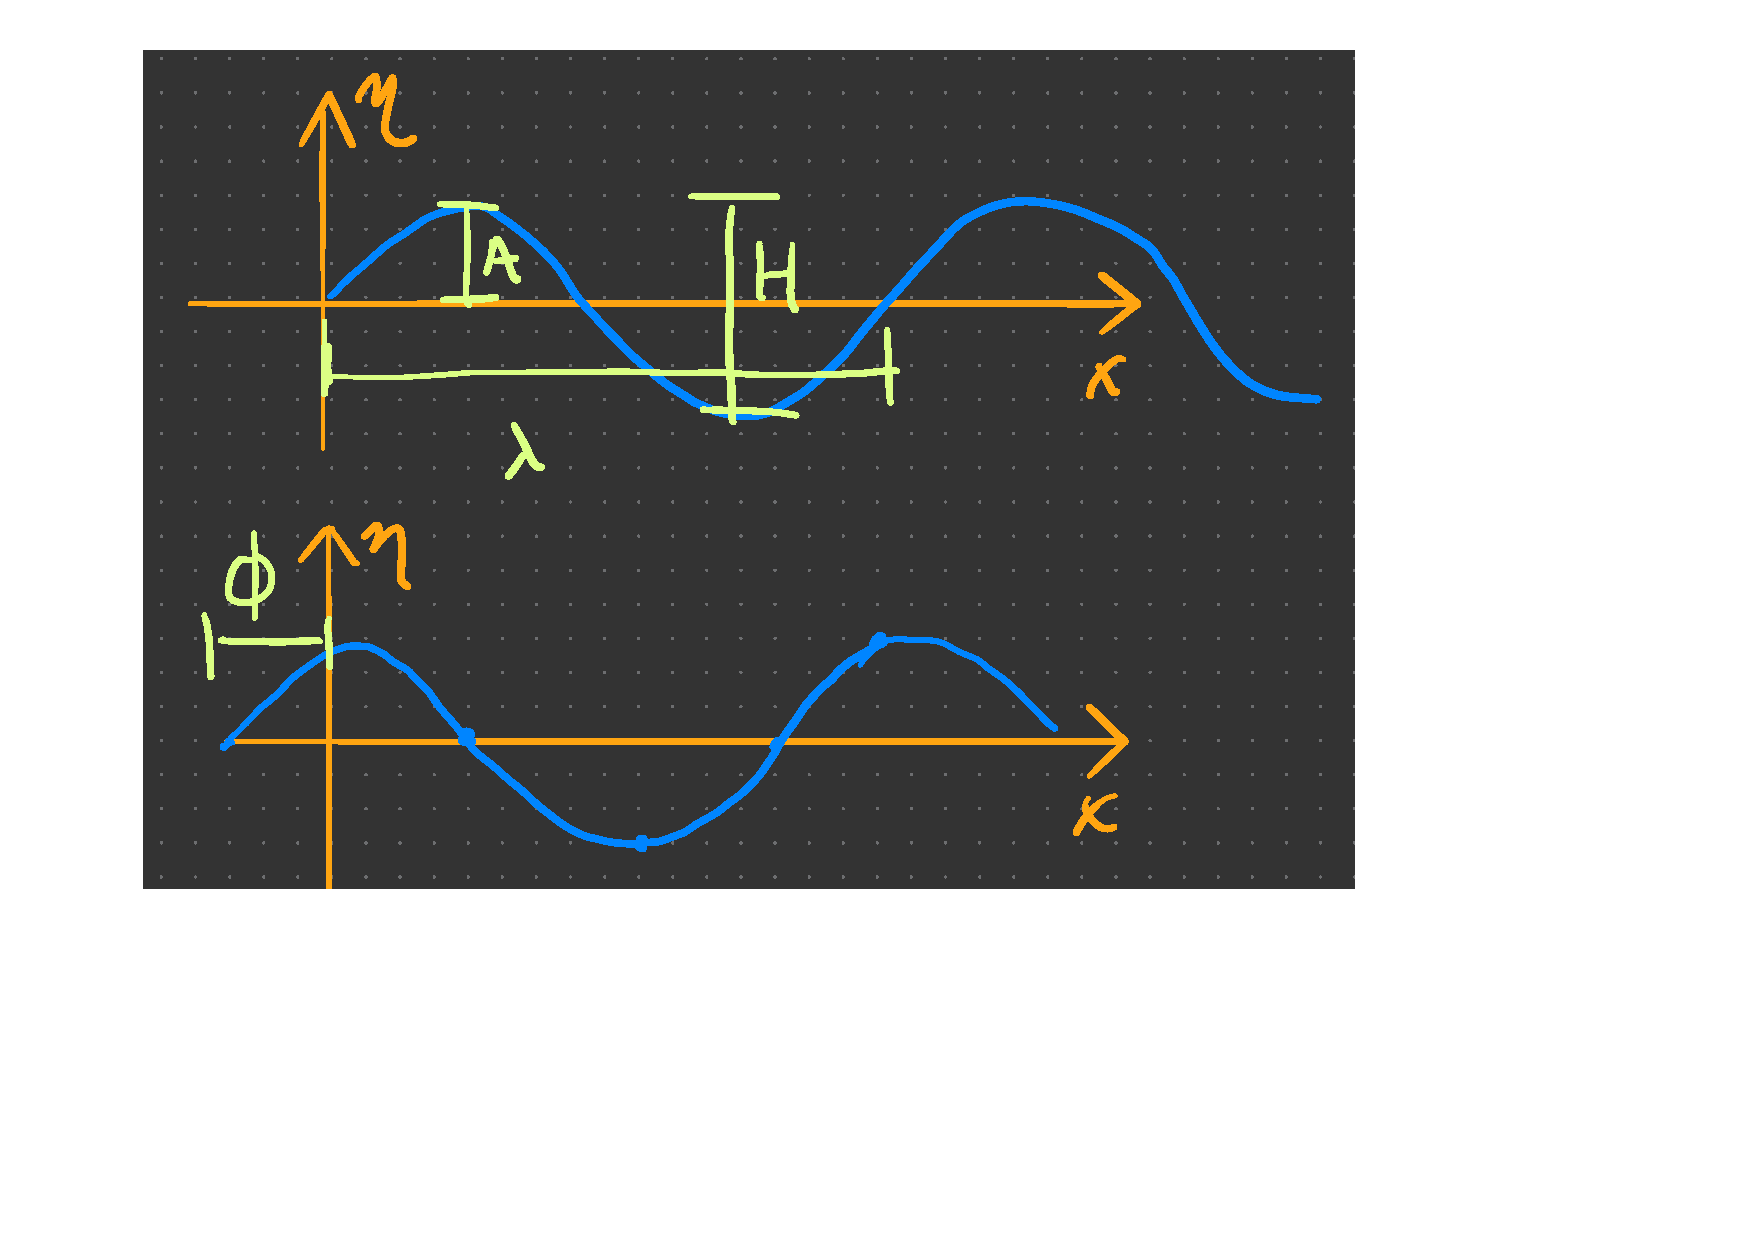
\includegraphics{figs/Waves/SketchDefnX}
    \caption{Sketch of sinusoidal wave forms that are frozen in time. The bottom sketch has a different phase $\phi$ than the top sketch. }
    \label{fig:SketchDefnX}  
\end{marginfigure}

To fully specify a wave on the surface of the ocean, we need two other pieces of information.  First, we need to specify where the crests are relative to where we define $x=0$.  That sounds abstract, but all it means is that we would like to know not only how high and far apart crests are, but also where they are at any given time.  Second, we need to know the direction the wave is travelling.  Usually, we will just consider waves travelling in one-dimension in the class, but bear in mind that in \fref{fig:SketchDefnX} the direction that $x$ points along is usually taken to be in the direction of wave propagation (or its opposite.  If we took it to be at a different angle, then the wave crests would appear further apart than they are in the direction of propagation (\fref{fig:SketchWaveAngle}).    

\begin{marginfigure}
  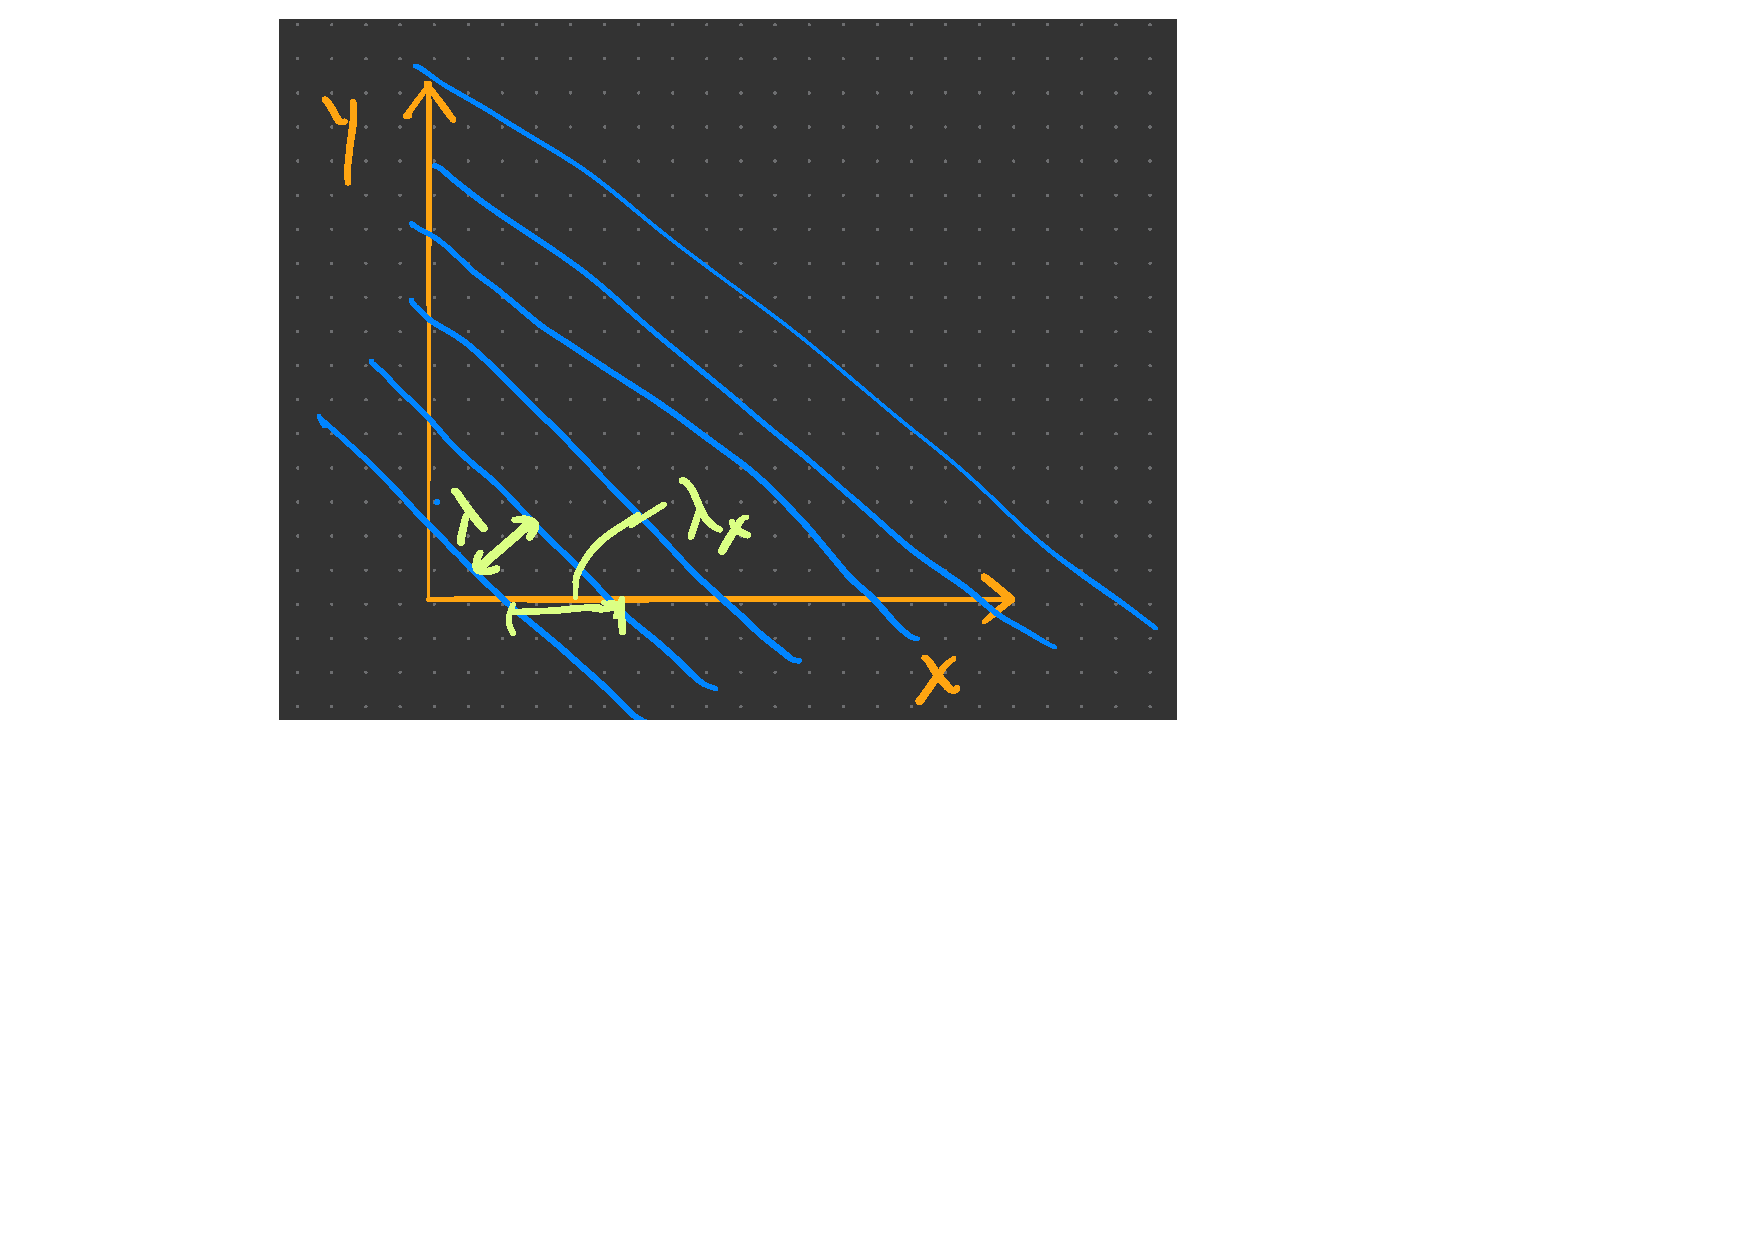
\includegraphics{figs/Waves/SketchWaveAngle}
    \caption{Schematic of wave crests at an angle to the "x" axis.  Note that the wavelength $\lambda$ is shorter than it would appear if we looked at the waves along the x axis $\lambda_x$}
    \label{fig:SketchWaveAngle}  
\end{marginfigure}

Mathematically, we therefore write the description of the sea surface displacement $\eta$ wave as $\eta(x) = A \sin \left( \frac{ 2\pi}{\lambda}x +\phi\right)$, where $\phi$ is the phase that describes where the zero crossing will be.  The term $\frac{2\pi}{\lambda}$ comes up all the time so we define $k = \frac{2\pi}{\lambda}$, where $k$ is called the \emph{wavenumber} and has units of $\mathrm{rad\,m^{-1}}$.  Using this shorthand, we see can rewrite the sinusoid as $\eta(x) = A \sin \left( kx +\phi\right)$.

Waves also have time dependence.  So if we were looking at one spot we would see the wave moving up and down such that it completes a complete cycle in one \emph{period}, which we usually denote with a $T$.  Mathematically, the time dependence can be written as $\eta(t) = A \sin \left( \frac{ 2\pi}{T}t +\phi_2\right)$, or in terms of an angular frequency $\omega = \frac{2\pi}{T}$ ($\mathrm{rad\,s^{-1}}$):  $\eta(t) = A \sin \left( \omega t +\phi_2 \right)$.  Note that if it is the same wave as we took the spatial snapshot of, then the amplitude $A$ will be the same in both frames of reference, but the phase $\phi$ will be different.  

This is two ways of looking at the same wave, so combining them, we say that 
\begin{equation}
  \eta(x, t) = A \sin ( kx - \omega t + \phi)
  \label{eq:propogatingwave}
\end{equation}
where $\eta(0, 0) = A\sin \phi$ is the height of the sea surface at $x=0, t=0$.  If the frequency is not zero, then the wave propagates in space. If $k>0$ then the wave will propagate to the right (\fref{fig:WaveHovmoller}).  Rather than drawing the curve many times, we can also plot as an \emph{Hovm\"oller diagram} and trace the crests as a series of highs and troughs as lows (\fref{fig:WaveHovmoller}).  The crests and troughs are examples of \emph{lines of constant phase} (as are the "nulls", coloured as white here), and for a wave in a homogenous medium they follow straight lines.  The slope of these lines is given by $T/\lambda$, and is inversely proportional to how fast the phases (e.g.\ the crests) of the wave move.  So, we say that the \emph{phase speed} of the wave is $c_P = \lambda / T$, or $c_P = \omega / k$.  

\begin{figure}[hbt]
  \begin{center}
  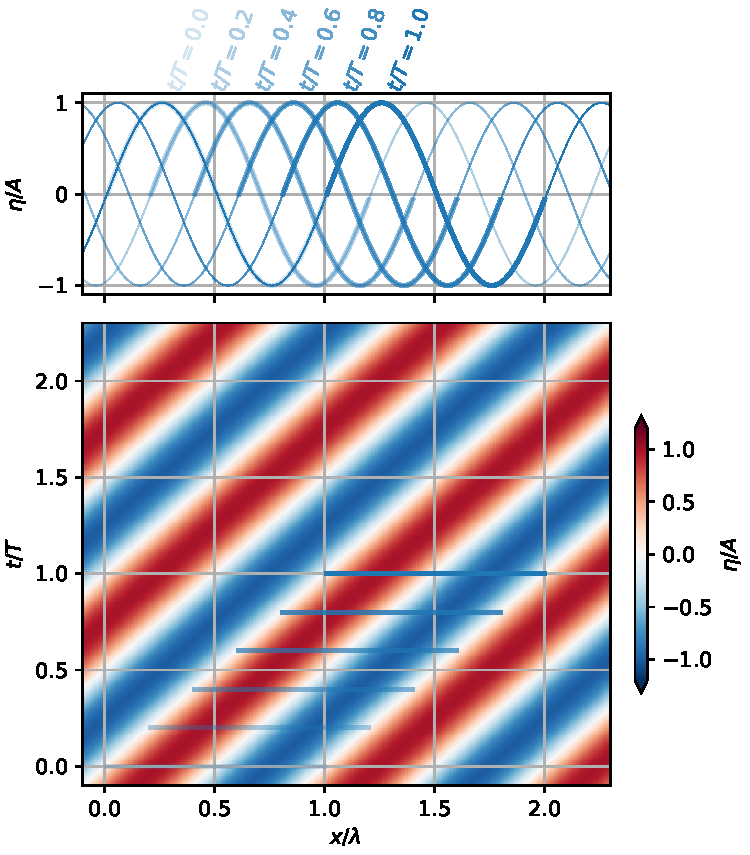
\includegraphics{figs/Waves/WaveHovmoller}
    \caption{Upper panel: Schematic of a propagating wave, where the trace gets darker as time progresses.  For this wave $k>0$, so the wave crests propagate to the right.  Note also that we have drawn this with $\phi=0$ if the wave is described by \fref{eq:propogatingwave}.  Lower panel: Hovm\"oller diagram of a wave propagating to the right in $x$.  Peaks of the wave are red, and troughs blue. Blue lines on this panel correspond to the thick blue traces on the panel above.   }
    \label{fig:WaveHovmoller}  
  \end{center}
\end{figure}


\section{Causes}

Waves are caused by some sort of unsteady forcing - if you wanted to make a wave in a bathtub, you would move your hand back and forth at a particular frequency.  This would raise and lower the water level in front of your hand, and then the wave would propagate away.  

In the ocean,  most waves are caused by the wind (tsunamis caused by earthquakes are thankfully rare).  The process by which waves develop is a continuum of processes, but the basic idea is that initially ``cat's paws'' develop making small \emph{capillary waves}.  These waves actually have surface-tension as a restoring force, and have wavelengths of the order centimeters.  On a calm day with small gusts of wind you can see these as local patches of roughness on the water.  

If the wind is sustained, resonances with some wavelengths will lead to a growth of those waves.  These resonances put energy in at all scales, but do so more efficiently at some, and waves with those wavelengths grow the fastest.  The simples way to think about the resonances is in terms of \emph{Jeffrey's sheltering theory}.  As waves grow in size, the flow on the upstream side is blocked by the wave, and the downstream side is ``sheltered'' by the wave (\fref{fig:SketchJeffreys}. This creates high pressure on the windward face and low pressure on the downwind side, and this acts to steepen the wave.  It is a resonance, because if the wave gets steeper, the effect grows stronger, and the wave continues to grow.  How quick this resonance is, and what wavelength waves are affected the quickest depend on the wind speed.  

\begin{marginfigure}
    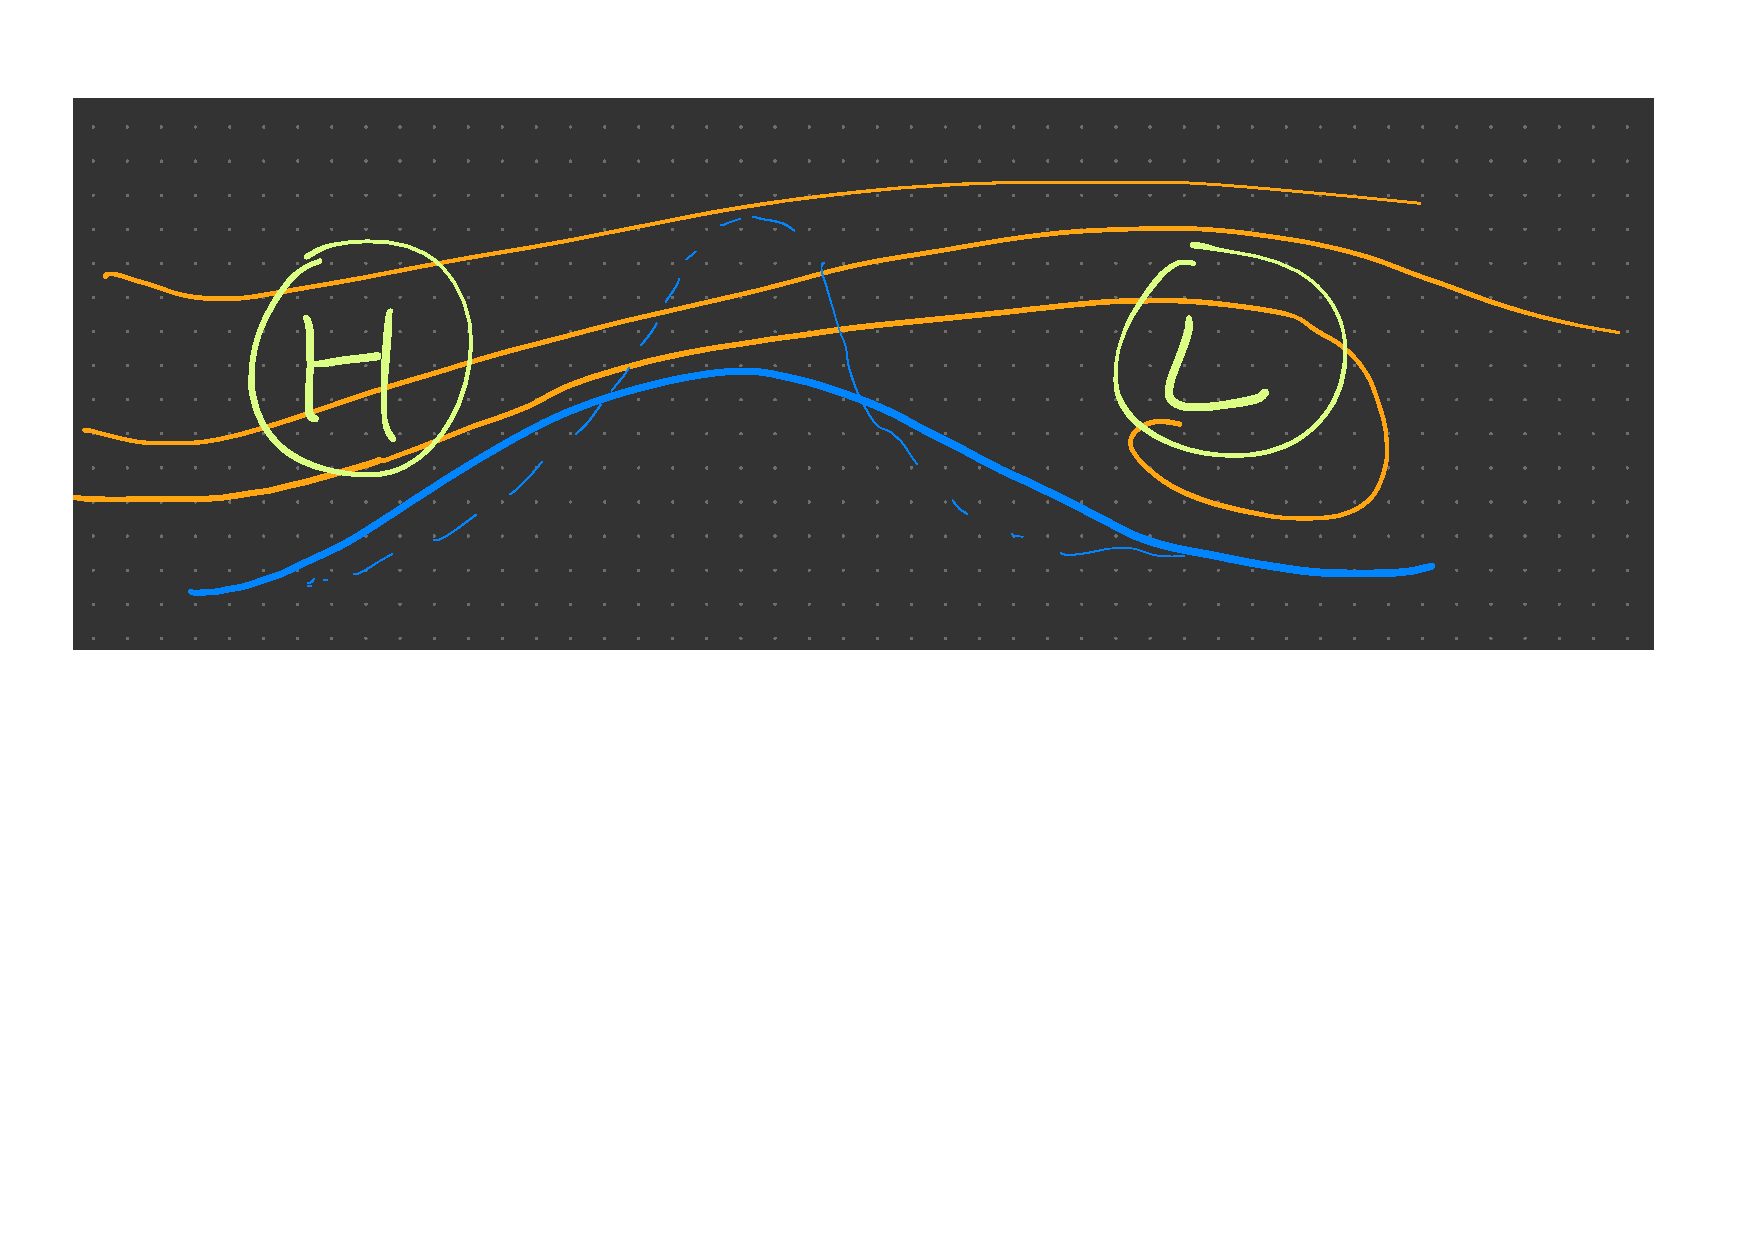
\includegraphics{figs/Waves/SketchJeffreys}
    \caption{Sketch of the streamlines of air over a relatively steep wave (orange) and the pressure difference they would experience. }
    \label{fig:SketchJeffreys}  
\end{marginfigure}


Waves are only able to grow to be so steep before they break.  the criteria for breaking in the open ocean is that the amplitude of the wave $A$ cannot be much more than 1/15th the wavelength of the wave.  This is actually quite large, and a 100-m horizontal scale wave will not break on its own unless its amplitude reaches 7 m or 14 m height.  Waves tend to break before this due to the wind pushing the crests over, or waves interacting with each other to produce localized breaking regions.  

Waves get larger, but also longer, as the wind speed increases.  That is because the shorter waves tend to break sooner, and dissipate out of the system.  A ``fully-developed'' sea is one in which the wind has been blowing a sufficiently long time that the waves have reached a steady state.  In that situation the ocean will take on characteristic wave sizes, and amounts of breaking (\fref{fig:SeaStatePics}).  

\begin{figure}[hbt]
  \begin{center}
    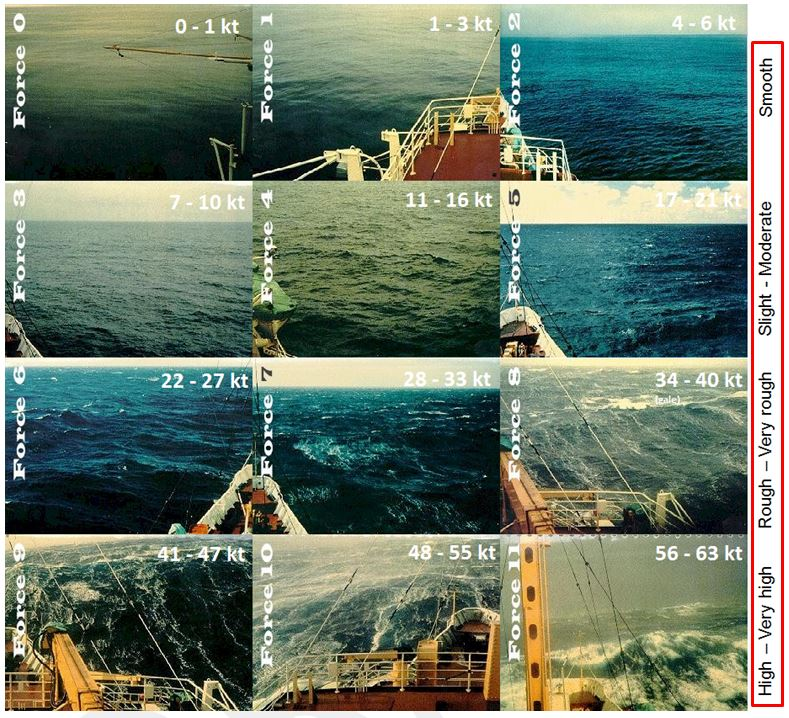
\includegraphics{figs/Waves/SeaStatePics}
    \caption{Pictures of fully-developed seas at increasing wind strengths.  }
    \label{fig:SeaStatePics}  
  \end{center}
\end{figure}

Of course waves have spatial dependence as well, just as the storms that make them have spatial dependence.  A snapshot from a model shows that the waves track the storms quite closely (\fref{fig:WaveHeightGlobal}), but you can also see bands of energy leaking North from  the southern ocean.  These are propagating waves, radiating energy from their source. (For a movie visit \url{https://csdms.colorado.edu/wiki/Movie:Global_Wave_Power_2012}.)  Indeed, the longest waves are the fastest (as we will see below), and can sometimes outrun the storms that create them.  We see this quite often on the West Coast, where swell will arrive a day or so before a winter storm.  

\begin{figure}[hbt]
  \begin{center}
      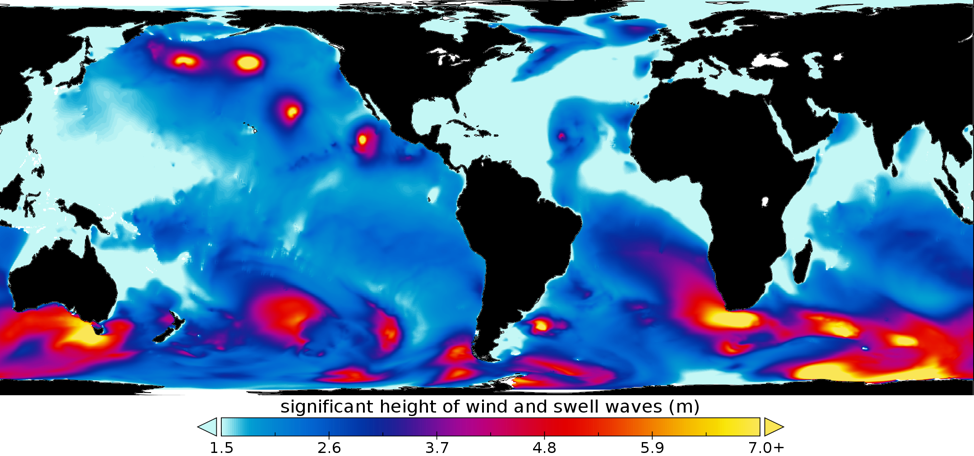
\includegraphics{figs/Waves/WaveHeightGlobal}
    \caption{Snapshot of global wave heights during the boreal summer.  }
    \label{fig:WaveHeightGlobal}
  \end{center}
\end{figure}

\section{Dispersion relation, phase speed, and particle motion}

So far we have discussed the wavelength and period of the wave like they are independent, but in reality they depend on each other.  Most people would expect that longer waves (large $\lambda$) will tend to have longer periods $T$.  You can try this at home with a bathtub or sink - the wavelength of the waves you make depends on the frequency you slash with, not with how far you move your hand or paddle.  

The relationship between the period and the wavelength is called the \emph{dispersion relation}, and depends on the properties of the fluid and the physics of the waves.  We are considering surface gravity waves, so of course this relationship depends on the strength of the gravity: $g = 9.8\ \mathrm{m\,s^{-2}}$. It also depends on the water depth, which we will call $h$, and the wavelength of the wave $\lambda$.  The general dispersion relation is a bit complicated:
\begin{equation}
  \omega^2  =  g k \tanh kh
\end{equation}
but it has two much simpler asymptotes that are applicable depending on the ratio of the wavelength to depth (or the product of $kh$ (\fref{fig:DispersionRelation}).    If $kh<<1$ then the waves are ``long'' compared to the water depth, or we can also call the ``shallow'' water.  In that case $\tanh kh \to kh$, and the dispersion relation is 
\begin{equation}
    \omega = \sqrt{gh}\ k    
\end{equation}
(blue line in \fref{fig:DispersionRelation}). The phase speed of these waves are all the same, and only depend on the water depth $c_p = \omega / k = \sqrt{gh}$. We see then from this that as waves move into shallower water waves will get slower.  


\begin{marginfigure}
 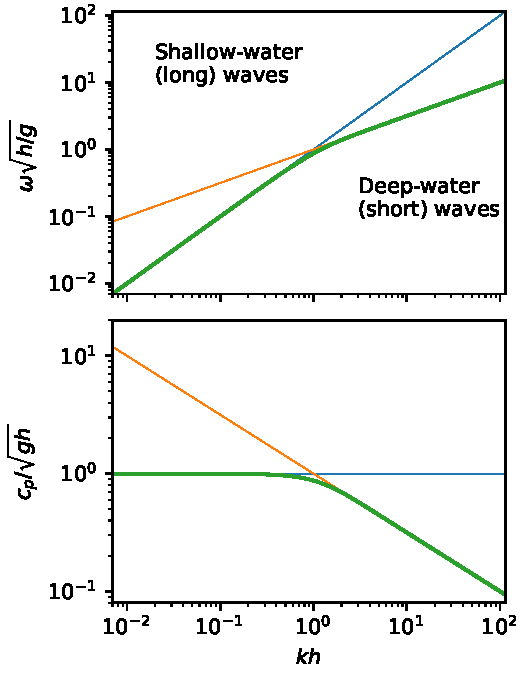
\includegraphics{figs/Waves/DispersionRelation}
    \caption{Upper panel: Dispersion relation for surface gravity waves (green), with the long-wave (blue) and short-wave (orange) asymptotes.  Note the logarithmic scale used. Lower panel: dispersion relation expressed as phase speed.   }
    \label{fig:DispersionRelation}  
\end{marginfigure}

Deep water waves are quite different.  They do not feel the bottom, so their phase speed only depends on the water depth.  As $kh>>1$, then $\tanh kh \to 1$ and 
\begin{equation}
  \omega = \sqrt{gk}    
\end{equation}
and hence their phase speed is $c_p = \sqrt{g/k}$.  So as $k$ gets larger, the wavelength of the waves is shorter, and they move more slowly.  


\section{Orbital motions: velocity of water parcels}

It is important to bear in mind that linear waves do not carry water with them.  Non-linear waves do, and much of our intuition is from beaches where waves obviously push the water up the beach.  But in open water where the waves are more likely to be linear, the water in a wave crest moves with the wave, but the water in the trough moves against the wave, so that over a wave period there is no net water motion. So while the wave crests move at the phase speed of the wave, the actual water does not move when averaged over a wave period. 

In deep water, the velocity induced by the waves decays with depth with a vertical scale proportional to $k^{-1}$.  So, longer wavelengths are felt to deeper depths (\fref{fig:SketchOrbitalVel}).  This is why when scuba diving you often do not feel the surface waves.    This also provides some physical justification for the different physics of ``deep'' versus ``shallow'' waves - deep waves do not feel the sea floor, whereas shallow ones do.  In deep water, parcels of water make perfect circles, but as the water gets more shallow these circles are compressed by the bottom and become ellipses, and eventually there is almost no vertical motion and the water just moves back and forth.  

\begin{figure}[hbt]
  \begin{center}
    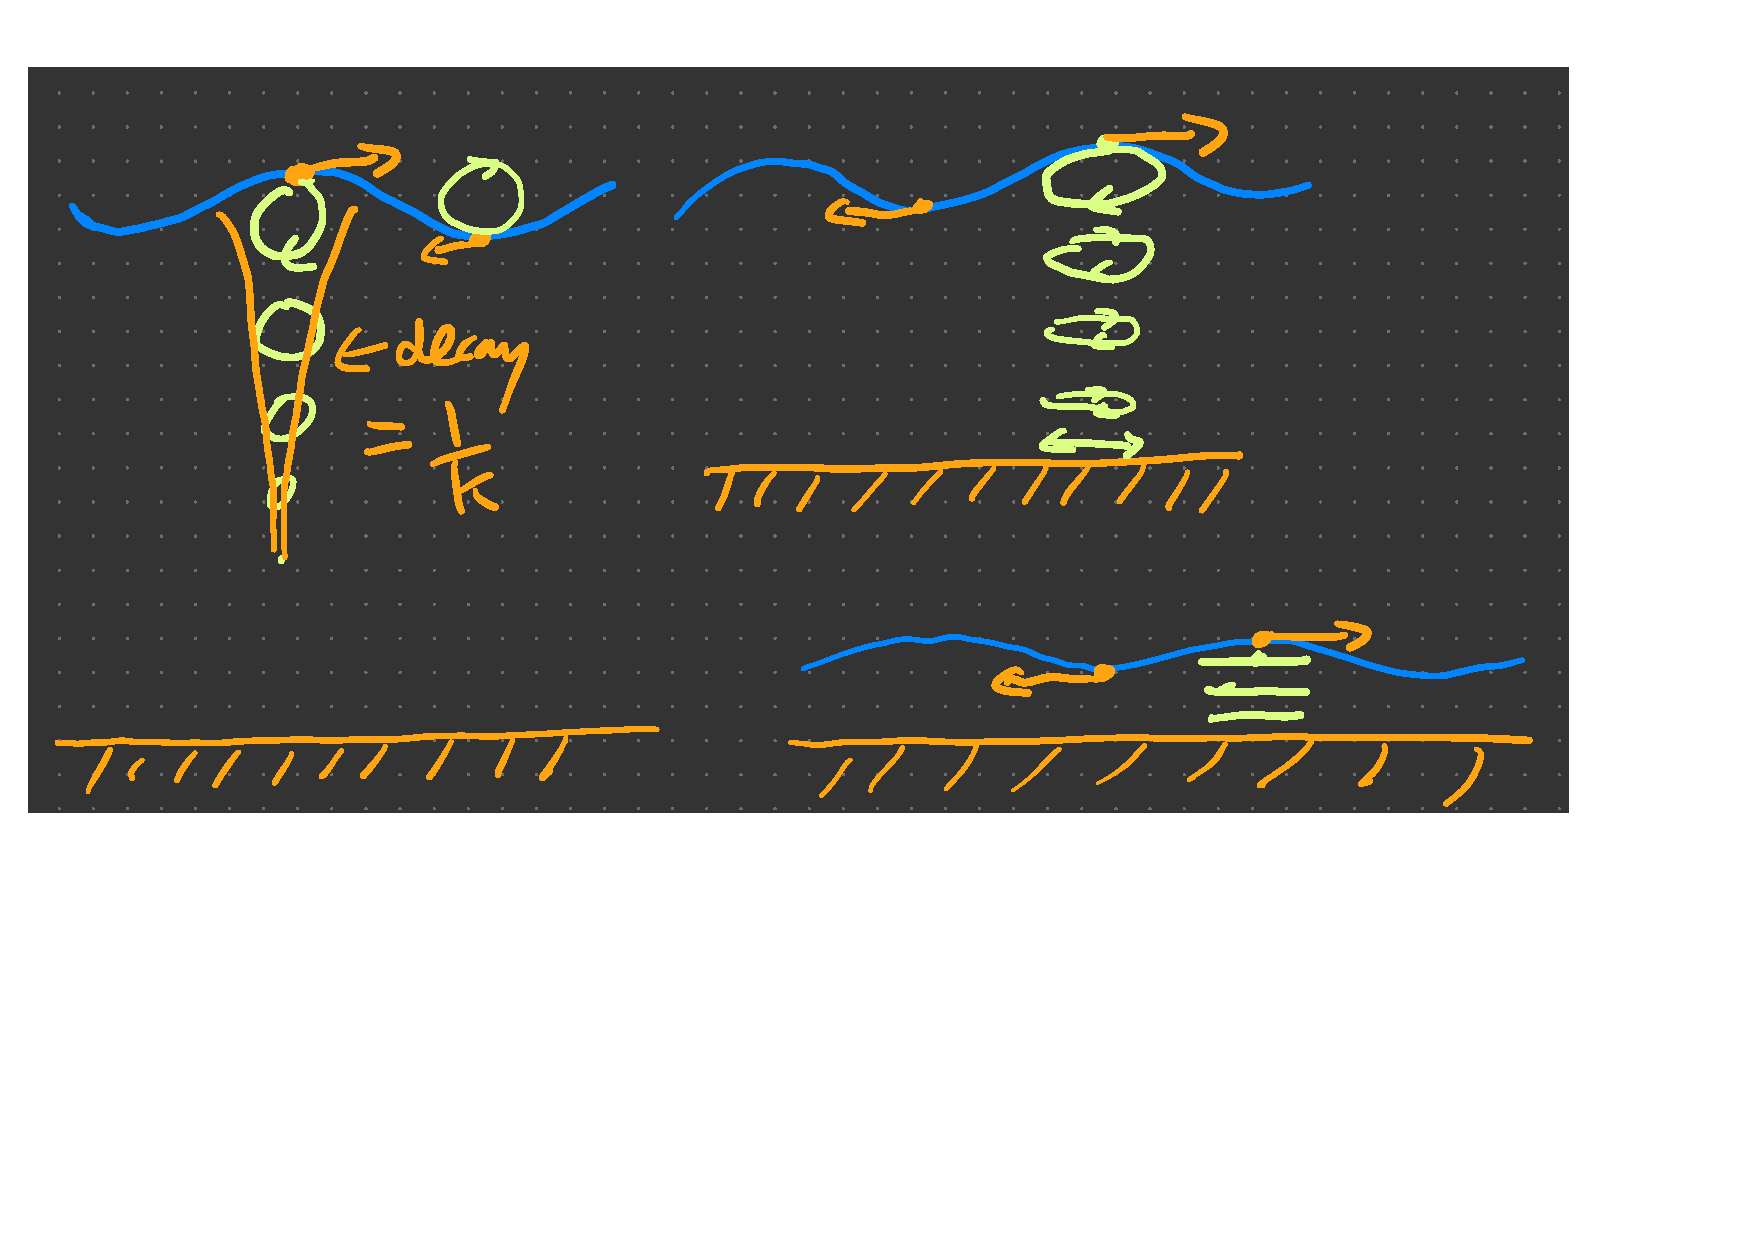
\includegraphics{figs/Waves/SketchOrbitalVel}
    \caption{Sketch of orbital velocities of waves in three different depths: deep, intermediate and shallow.}
    \label{fig:SketchOrbitalVel}  
  \end{center}
\end{figure}

Thinking about the velocity of water parcels also helps us understand why waves propagate.  The flows are in opposite directions beneath the crest and the trough, and hence there is a convergence there (\fref{fig:SketchesWaveConvergence}), and the peak moves in the direction of the flow under the crest.  Note that for a left-going wave the flow direction under the crest is to the left, and the same argument applies.  

\begin{figure}[hbt]
  \begin{center}
    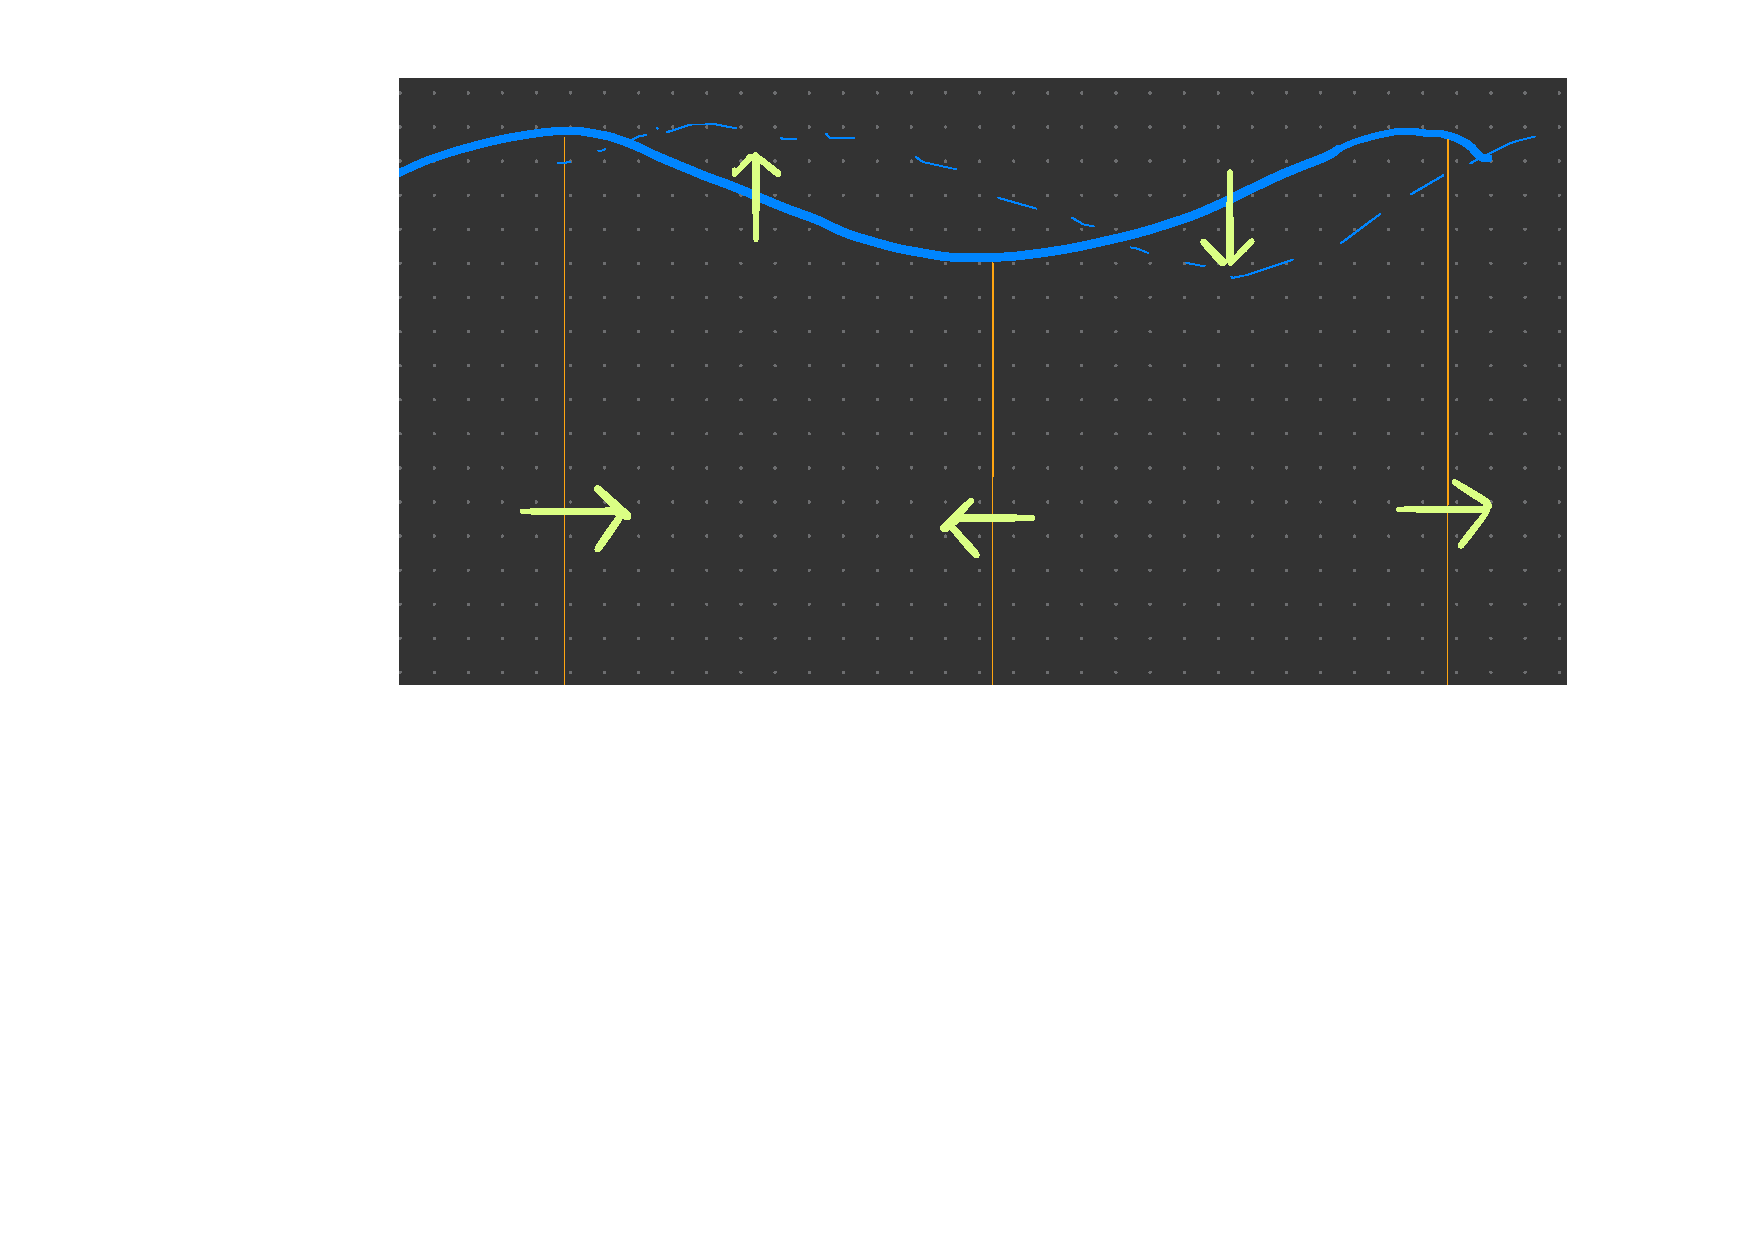
\includegraphics[width=3in]{figs/Waves/SketchesWaveConvergence}
    \caption{Sketch of how convergence and divergence in a wave causes it to propagate.}
    \label{fig:SketchesWaveConvergence}  
  \end{center}
\end{figure}

\section{Group speed}

% Todo: get image...

Deep-water waves (or short waves) are examples of \emph{dispersive} waves, in that the longer wavelengths and lower frequencies travel faster than the shorter.  This leads to interesting effects when we consider packets or \emph{groups} of waves.  

A sine-wave describes an infinite disturbance - the wave oscillates for ever and for all values of $x$.  Of course real wave packets or \emph{groups} are finite in extent because the storms that make them are finite.  One way to make a group of waves is to add together many sine waves with different amplitudes, wavenumbers, and phases, so that they \emph{interfere} with one another such that when you add them together, they make a group.  The simplest group occurs when we add two sine waves together with different wavelengths, and equal amplitudes.  This creates infinite repeating groups, but is the easiest way to get the idea (\fref{fig:InterferingWavesNonDisp}).  The waves in this figure have two slightly different wavelengths, and they are in 3.5 m of water, so the $\lambda > h$ and the phase speed of the waves is $\sqrt{gh} = 5.9\ \mathrm{m\,s^{-1}}$.  Adding these two waves together gives peaks and nulls as the waves constrictively and destructively interfere with one another.

After 25s, both waves crests have travelled at 147 m at their phase speed.  The crests are still in phase, and so the group has also moves 147 m.  Because the waves stay in phase, we say they are \emph{non-dispersive}.  

\begin{figure}[hbt]
  \begin{center}
    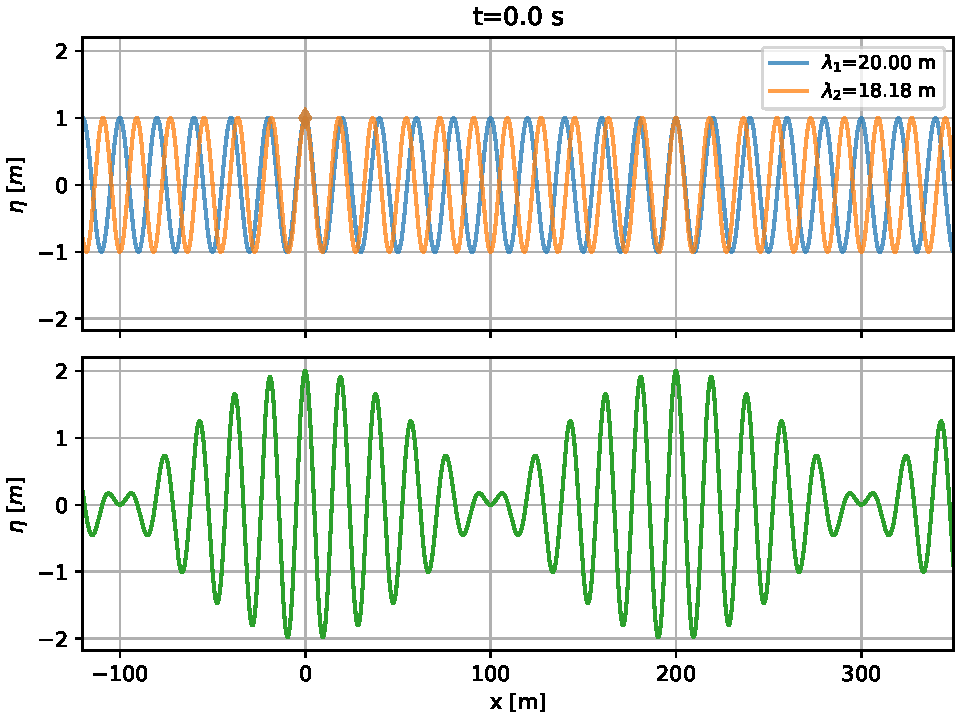
\includegraphics[width=3in]{figs/Waves/InterferingWavesNonDisp00.pdf}
    \includegraphics[width=3in]{figs/Waves/InterferingWavesNoNDisp25.pdf}
    \caption{Two non-dispersive waves added together to make group.  The crests are in phase at $x=0$ at $t=0$.  25 s later, both crests have traveled the same distance, and the ``group'' has moved with them.}
    \label{fig:InterferingWavesNonDisp}  
  \end{center}
\end{figure}

Conversely, consider two deepwater waves with the same wavelengths.  Here the phase speed is faster for the longer wave ($c_1 = \sqrt{ g \lambda_1 / 2 \pi} = 5.6\ \mathrm{m\,s^{-1}}$) compared to the shorter ($c_2 = 5.3\ \mathrm{m\,s^{-1}}$).  That means that after 25 s they have travelled 140 m and 132.5 m respectively, and moved 7.5 m out of phase (\fref{fig:InterferingWaves}).  This means that when we add the two waves together, the peak in the interference pattern has fallen behind the two waves that made the peak in the first place.  Hence, for \emph{dispersive waves} the group speed is different than the phase speed. In the case of deep-water waves is exactly half the phase speed, and we can clearly see that the peak of the group is at about 70 m, whereas the original wave crests are at about 140 m.  

\begin{figure}[hbt]
  \begin{center}
    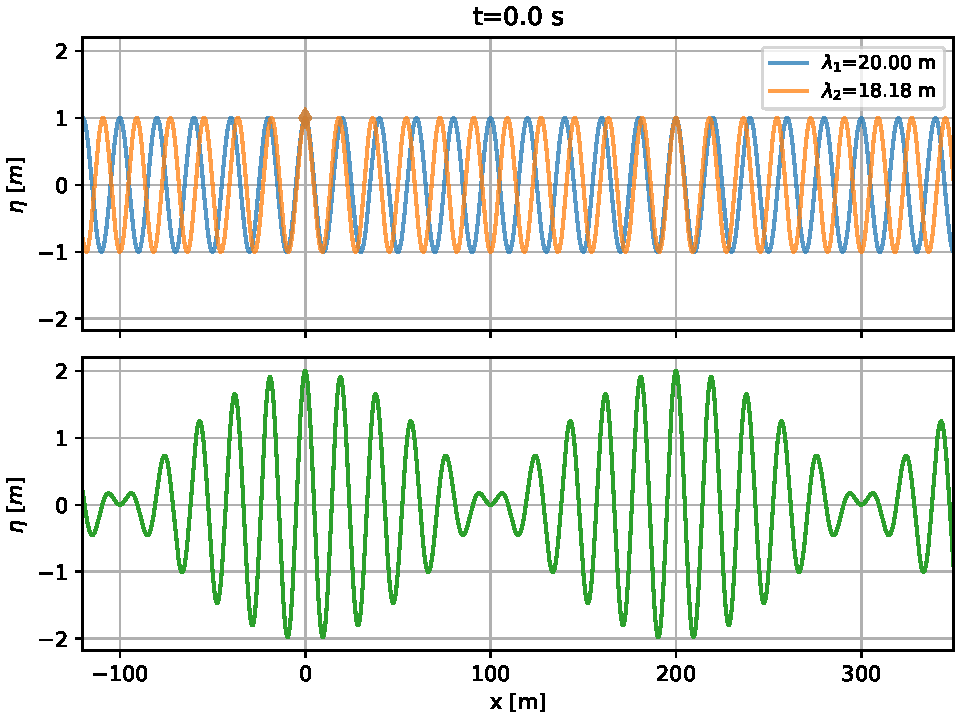
\includegraphics[width=3in]{figs/Waves/InterferingWaves00.pdf}
    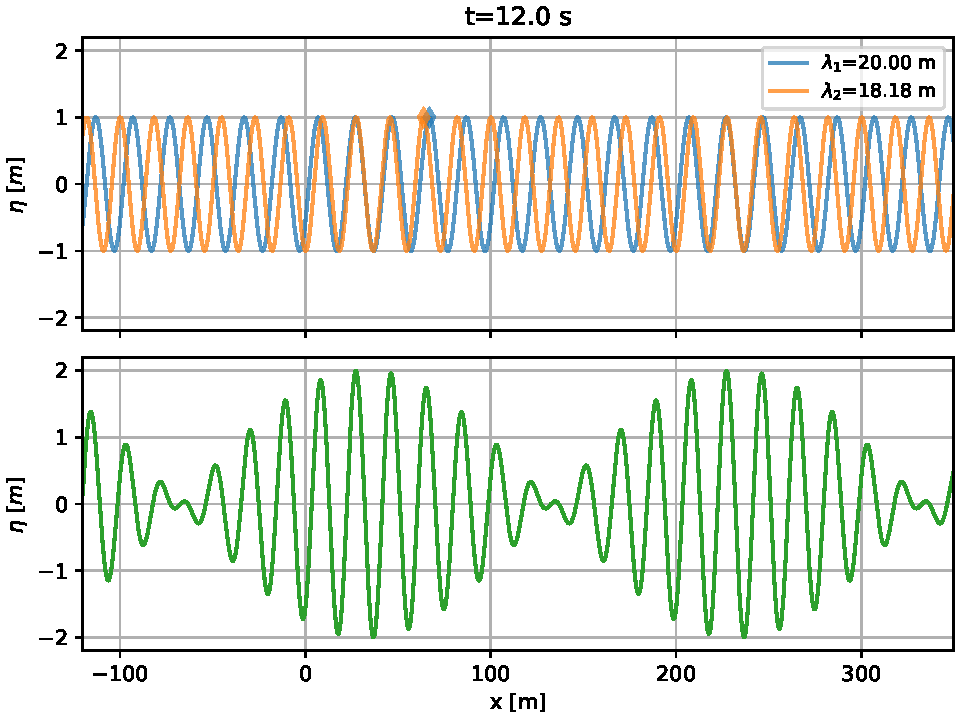
\includegraphics[width=3in]{figs/Waves/InterferingWaves12.pdf}
    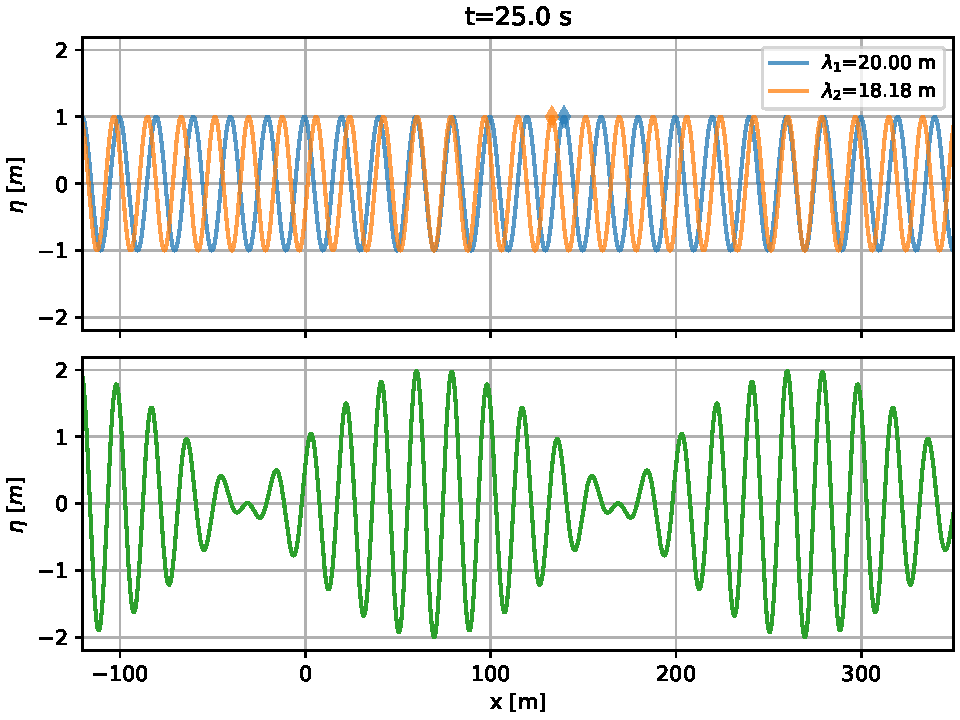
\includegraphics[width=3in]{figs/Waves/InterferingWaves25.pdf}
    \caption{wo non-dispersive waves added together to make groups.  The crests are in phase at $x=0$ at $t=0$. However, the longer wave moves faster than the shorter, and the crests move out of phase (diamonds), hence the interference pattern between the two falls back.}
    \label{fig:InterferingWaves}  
  \end{center}
\end{figure}

The speed of the group is given by the derivative of the dispersion relation: $c_g = \frac{d\omega}{dk}$ which is called the \emph{group speed}.  

\begin{table}[hbt]
  \begin{tabular}{l|ccc}
    &long  (shallow water) & all waves& short (deep water) \\
    \hline
    dispersion & $\omega = k \sqrt{gh}$ & $\omega^2 = g k\tanh kh$  &  $\omega = \sqrt{gk}$ \\
    phase speed ($c_p$)& $\sqrt{gh}$ &  $\sqrt{g/k}\tanh^{1/2} kh$ & $\sqrt{g/k}$ \\
    group speed ($c_g$) & $c_p$& $\frac{c_p}{2}\left(1 + \frac{2kh}{\sinh{2kh}}\right)$   & $\frac{c_p}{2}$ 
  \end{tabular}
\end{table}

\begin{derivbox}[label={box:groupspeed}]{Derivation of group speed}
    The group speed is given by $c_g=\frac{d\omega}{dk}$ which can easily be seen by considering the summation of two sine waves with slightly different wavelengths (and hence frequencies):
\begin{eqnarray*}
    \eta &=& A \sin \left( (k+\delta k) x - (\omega + \delta\omega)t\right) +\\
    && A \sin \left( (k-\delta k) x - (\omega - \delta\omega)t\right) 
\end{eqnarray*}
Using the angle identity $\sin\theta + \sin\phi = 2\sin\left(\frac{\theta+\phi}{2} \right)\cos\left(\frac{\theta+\phi}{2} \right)$ we get
\begin{eqnarray*}
    \eta &=& 2A \sin \left( k x - \omega t\right)  \cos \left( \frac{\delta k}{2} x  - \frac{\delta \omega}{2} t\right)
\end{eqnarray*}
and we see that the combination of the waves is a convolution of a carrier wave with wavenumber $k$, frequency $\omega$ and an envelope with wavenumber $\delta k / 2$ and frequency $\delta \omega / 2$.  
\begin{center}
  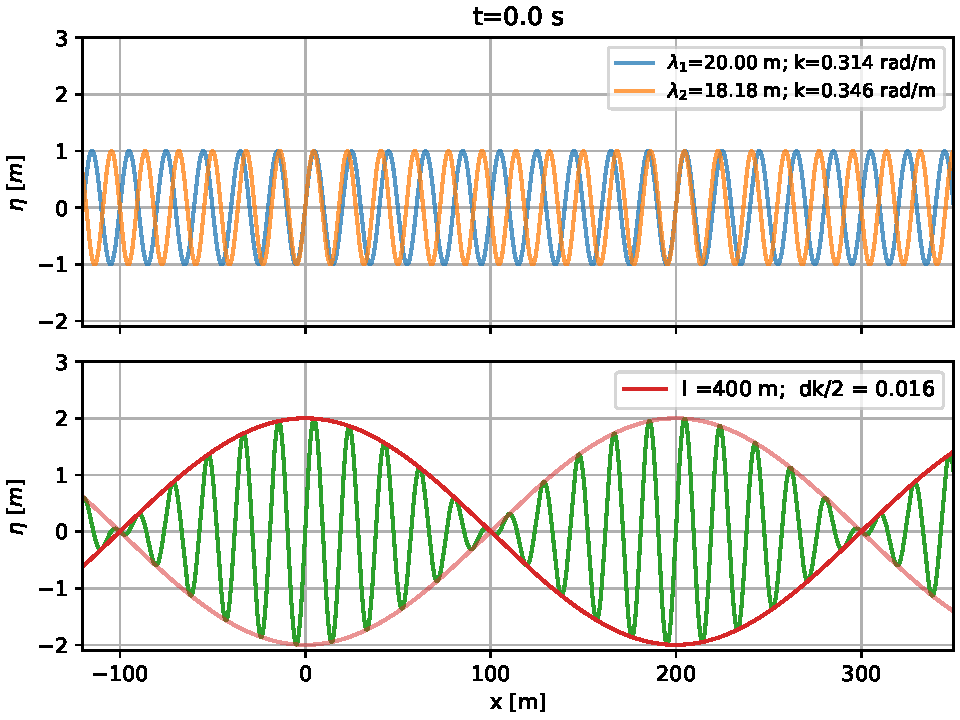
\includegraphics[width=3in]{figs/Waves/InterferingWavesEnvelope}
\end{center}
This envelope is the group, and propagates with speed $c_g=\delta \omega / \delta k \to \frac{d\omega}{dk}$
\end{derivbox}

Seeing the difference between the two types of waves is another useful application of a H\"ovmoller diagram (\fref{fig:Hovmoller}).  For the non-dispersive waves we can easily see that the crests of the individual waves follow the group, whereas for the deep-water dispersive waves, the group is propagating at half the speed.  

\begin{figure}[hbt]
  \begin{center}
    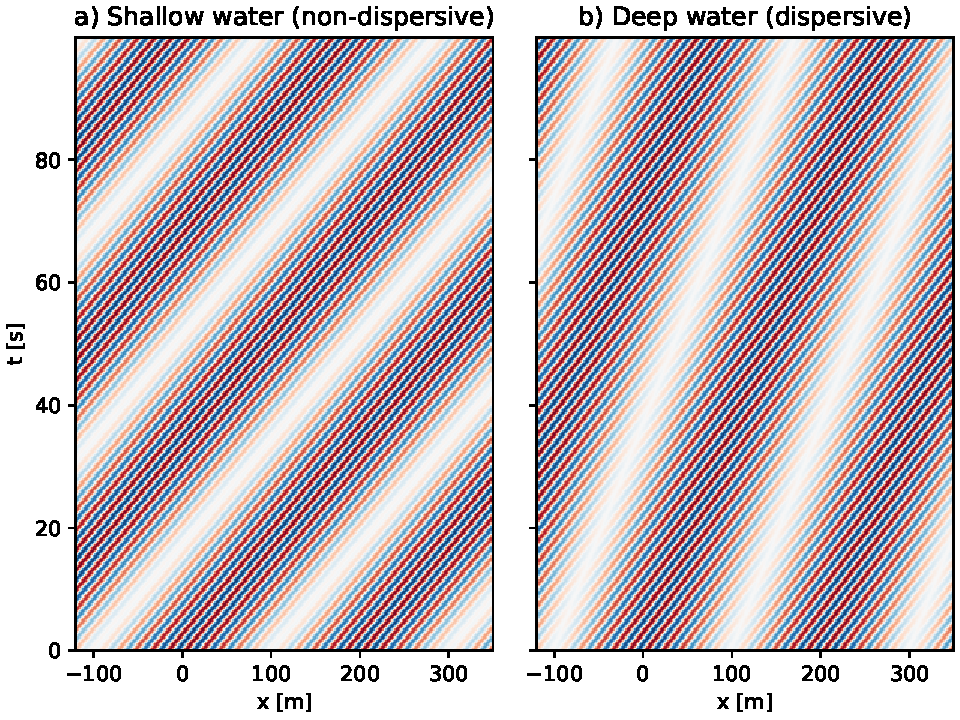
\includegraphics{figs/Waves/Hovmoller}
    \caption{a) H\"ovemoller diagram for two shallow water, non-dispersive waves with the same wavelengths as \fref{fig:InterferingWavesNonDisp} b) for deep-water dispersive waves (same two as \fref{fig:InterferingWaves}).}  
    \label{fig:Hovmoller}  
  \end{center}
\end{figure}

In the real ocean, the packets do not repeat like they do when we just add two waves together.  A more isolated group can be created if we consider summing together even more wavenumbers.  The same group speed applies, but since longer waves have a faster group speed, the packet will spread with time as the longer waves outrun the shorter (\fref{fig:DispersiveHov}).  

\begin{figure}[hbt]
  \begin{center}
    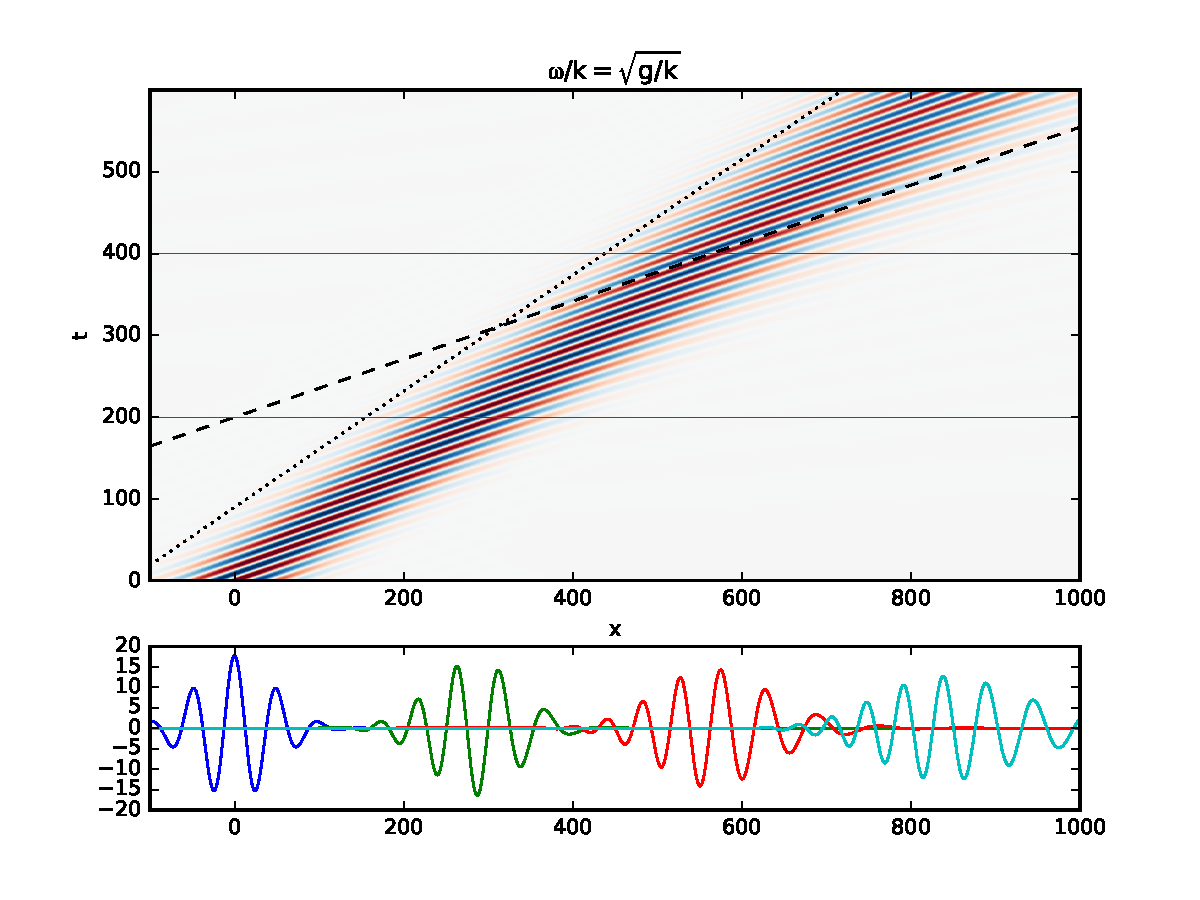
\includegraphics{figs/Waves/DispersiveHov}
    \caption{A very localized wave packet in deep water.  Note how the group ``disperses'' as time goes forward, and that the larger wavelengths are at the front of the packet, and shorter at the back.  }
    \label{fig:DispersiveHov}  
  \end{center}
\end{figure}

Note that for dispersive waves, there is the un-intuitive phenomena that wave crests and trough emerge from the back of the packet, move faster than the packet and then disappear at the front of the packet. This is unintuitive, but is fundamentally because waves are not particles, but the result of convergences and divergences. These convergences and divergences simply get weaker towards the front of the packet until they are gone.  

\clearpage

\section{Energy conservation}

Parcels of water are not carried by the waves, but \emph{energy} is definitely carried by the waves.  The speed at which the energy is carried is the group speed, as should be obvious by the fact that the disturbance created by the waves moves at that speed.  If the speed of the energy is $c_g$, then we need only know the energy density to get a flux or transport due to the waves.  

The energy density of waves is usually averaged over a period or wavelength.  Within a period or wavelength the wave energy peaks twice, once at the crest and once at the trough, both times when there is potential energy (because the water is displaced) and kinetic energy (because the water is moving).  We cannot derive the average energy density here, but for linear waves it is, per surface area of the ocean:
\begin{equation}
  E = \frac{1}{2} \rho g A^2  \ \ \ \ \mathrm{[J\ m^{-2}]}
\end{equation}
where remember that $A=H/2$ is the amplitude of the waves, and $\rho$ is the density of the water.  The energy flux is then 
\begin{equation}
  F = c_g E \ \ \ \ \mathrm{[W\ m^{-1}]}
\end{equation}
where this is the flux per meter perpendicular to the direction the waves are travelling.  

Considering the conservation of energy helps us understand some behaviour of waves as they are concentrated, either in shallower water or as a water way narrows.  In both cases the energy density must increase to to account for the reduced ability of the water to transport the waves.  

So, for the first case, suppose we have a shallow-water wave propagating from  $h_1 = 50 \mathrm{m}$ of water to a region where the water is only $h_2=10 \mathrm{m}$ deep.  If we assume there is no energy loss between the two water depths, then the \emph{fluxes} are equal, and 
\begin{equation}
     c_{g_1} E_1 = c_{g_2} E_2
\end{equation}
or,
\begin{equation}
    E_2 = \sqrt{\frac{h_1}{h_2}} E_1
\end{equation}
from which we get that the amplitude in the shallower water has increased
\begin{equation}
  A_2^2 = \sqrt{\frac{h_1}{h_2}} A_1^2
\end{equation}
because $\sqrt{\frac{h_1}{h_2}}  = \sqrt{5} > 1$.  Of course we see this at the beach, where very small swell in deeper water amplifies and steepens as it reaches shore (e.g.\ \fref{fig:ParacasNational}). 

\begin{figure}[hbt]
  \begin{center}
    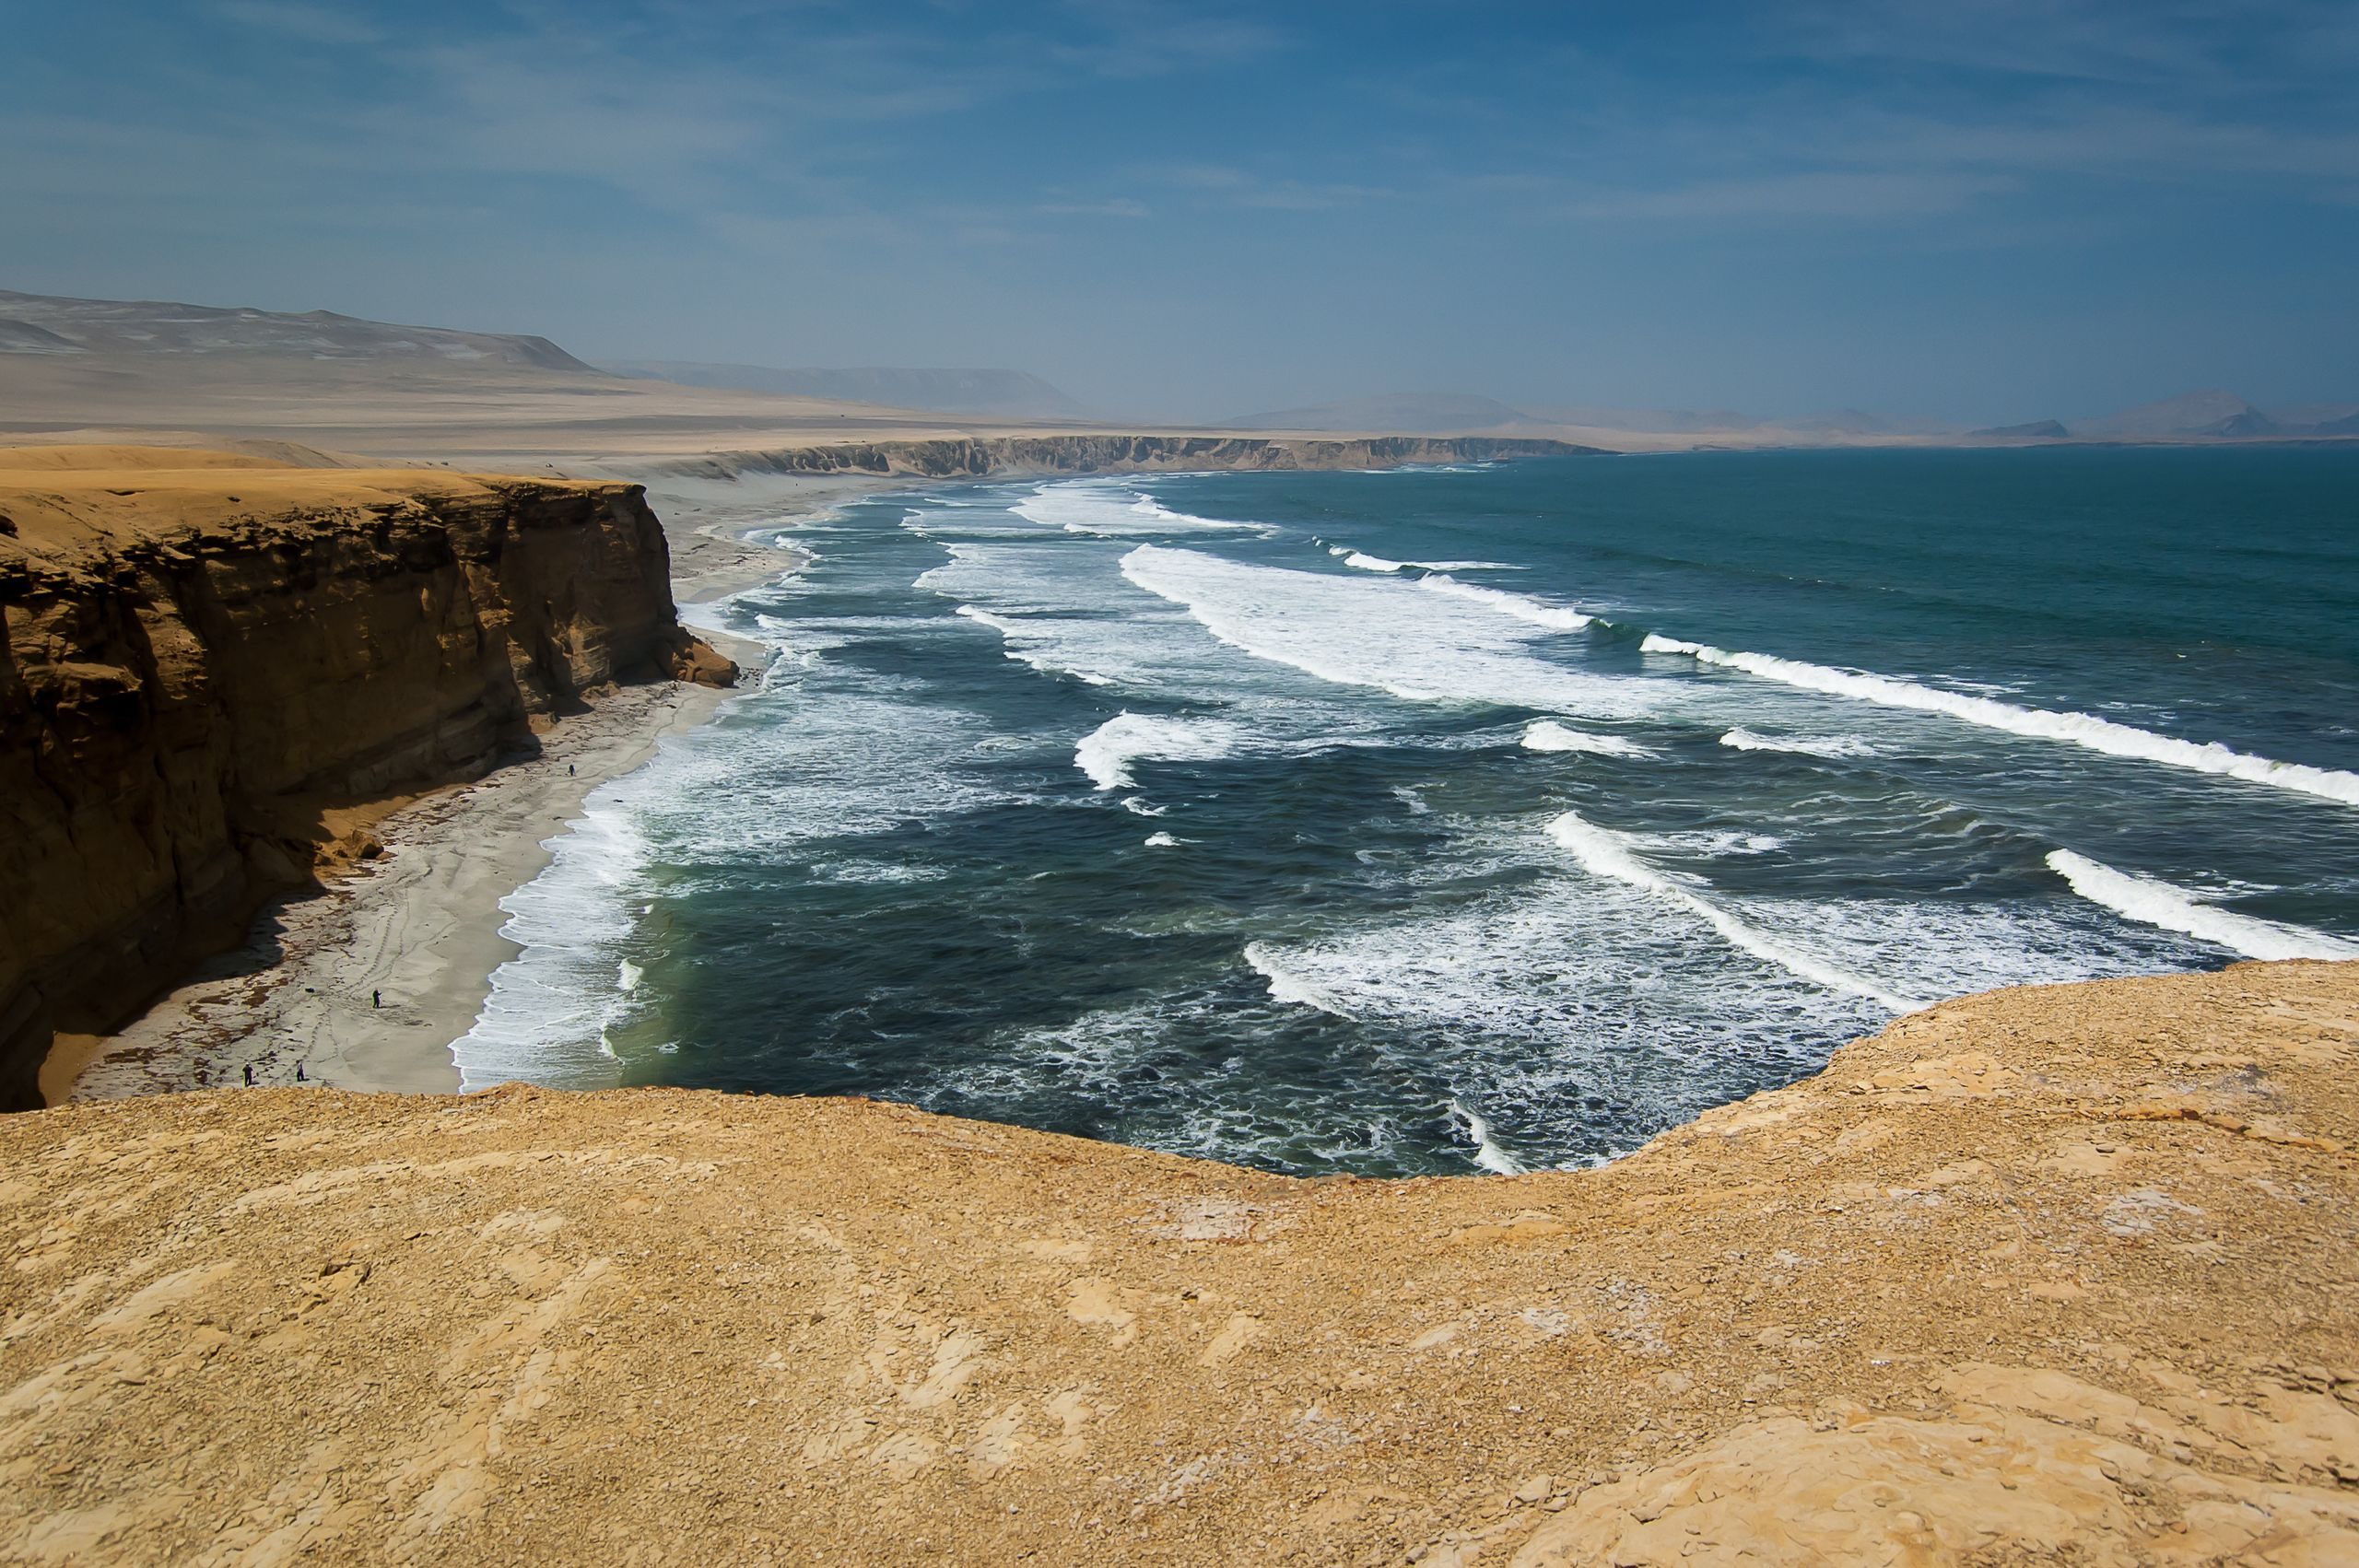
\includegraphics{figs/Waves/Paracas_National_Reserve,_Ica,_Peru-3April2011}
    \caption{Waves approaching a beach.  Note how offshore it is hard to see any waves (though of course its also further away).  \href{https://commons.wikimedia.org/w/index.php?title=File:Paracas_National_Reserve,_Ica,_Peru-3April2011.jpg&oldid=414758987}{Wikipedia}}
    \label{fig:ParacasNational}  
  \end{center}
\end{figure}

A similar concentration of energy will happen in a narrowing channel (\fref{fig:NarrowChannel}), even if the water depth stays constant.  In this case we need to take into account the width of the channel, which is perpendicular to the wave propagation, to get:
\begin{equation}
  W_1 F_1 = W_2 F_2\  \ \ \mathrm{W}
\end{equation}
But because $c_g$ is constant in this case,
\begin{equation}
    A_2^2 = \frac{W_1}{W_2} A_1^2   
\end{equation}
and, again, if $W_1 > W_2$, then $A_2 > A_1$ and the amplitude must increase.  

\begin{marginfigure}
    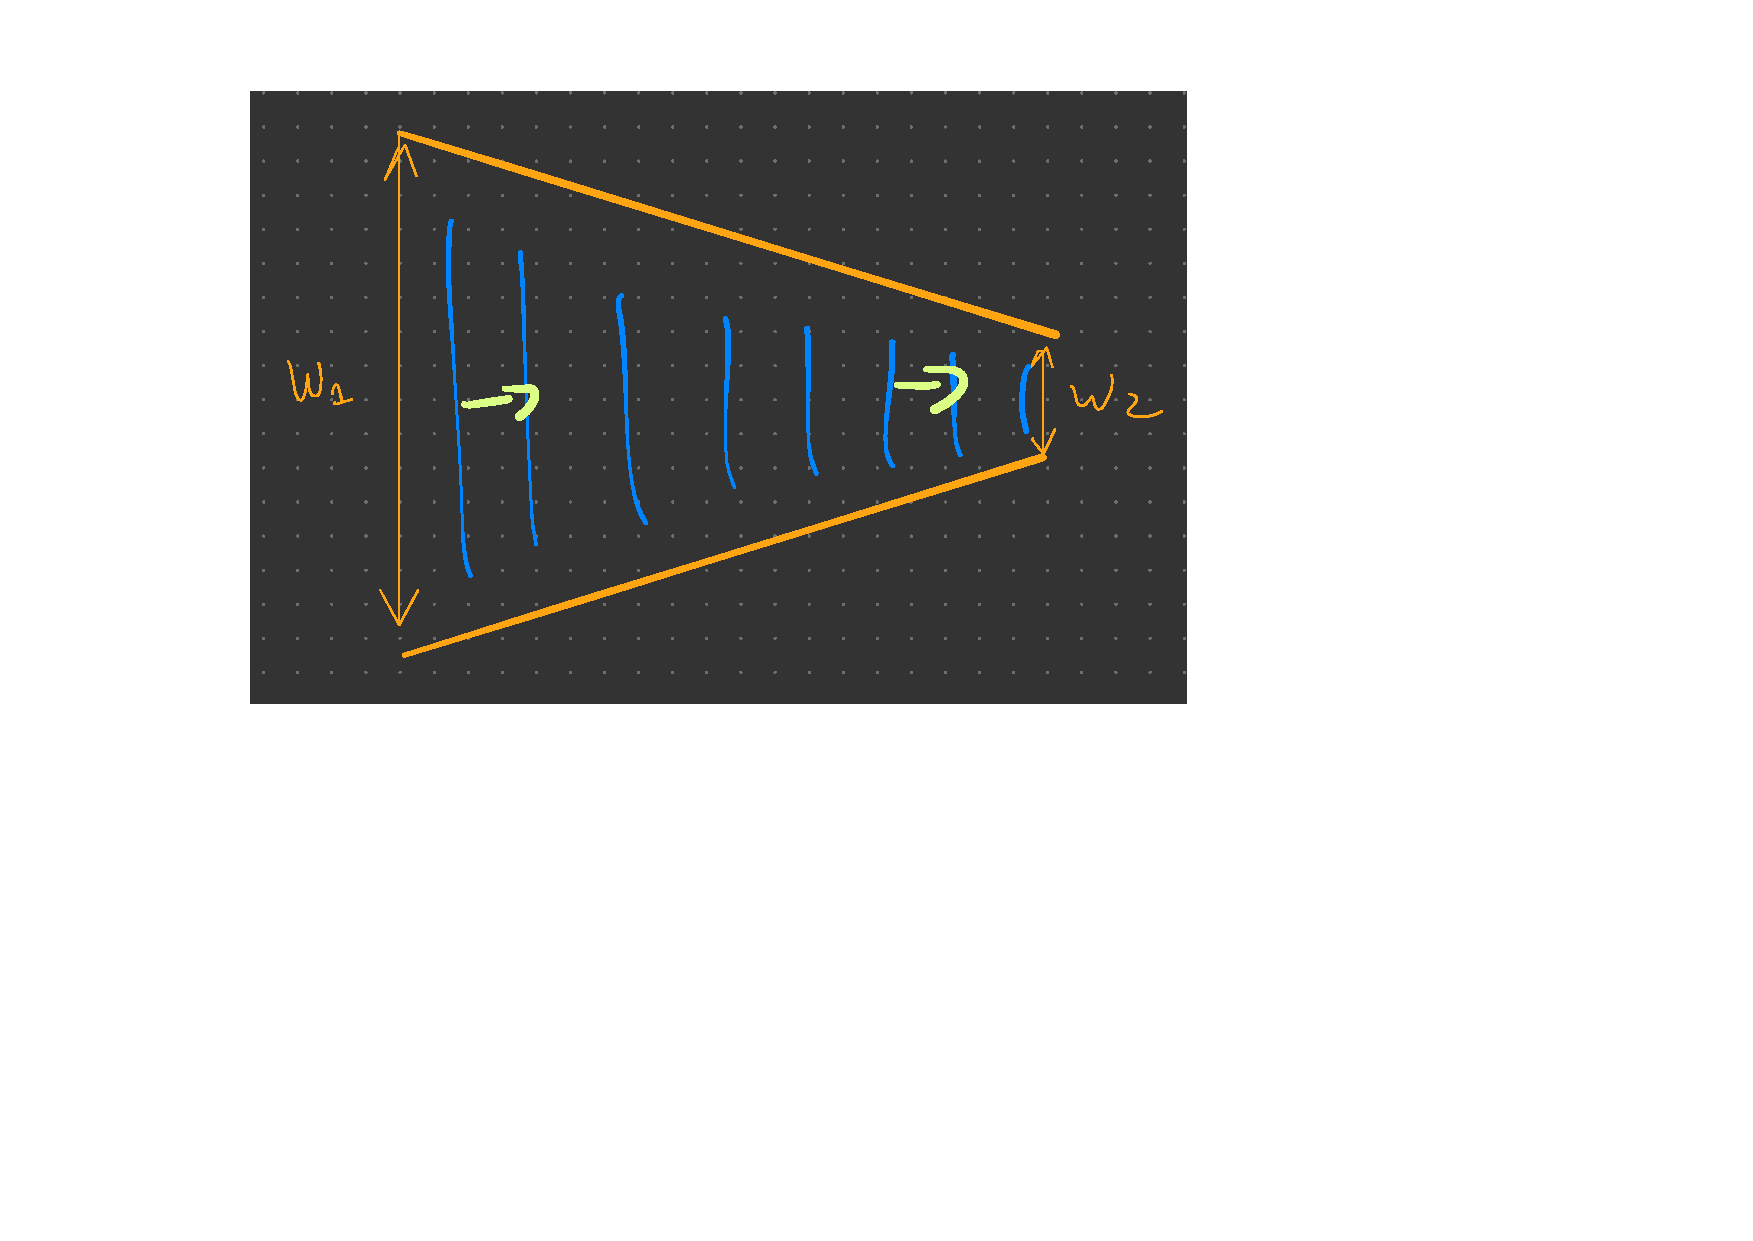
\includegraphics{figs/Waves/NarrowChannel}
    \caption{Waves propagating into a narrowing channel}
    \label{fig:NarrowChannel}  
\end{marginfigure}

One small note here is that in order for these energy relations to be easy to follow like this, the change of the bathymetry or the width of the channel must be gradual relative the the wavelength of the waves.  If it is not, then there will be some reflection from the bathymetry and wave energy will bounce backwards. Of course energy is still conserved, but you can end up with a partially standing wave.  


\section{Refraction and diffraction}

When standing at the seashore, waves are almost always coming towards the beach, and this is because of \emph{refraction}, the tendency of a wave to turn towards regions where the wave moves more slowly.  Because shallow water wave phase speed depends on the square root of the water depth, waves in shallower water move more slowly than they do in deeper water.  

Consider a wavefield heading towards a shoreline at an oblique angle (\fref{fig:RaytraceStraight}).  In order to stay in a straight line all parts of the wavefront must move at the same speed.  
However, the shoreward end of the waves hits the shallow/slow part of the water first and slows down and falls behind the straight line, bending the line with the wavecrests towards the shoreline  This continues to happen, and if the change of bottom depth is gradual enough the waves will eventually be parallel to the shore. Of course if the beach is quite steep, this won't happen perfectly, but the tendency is usually there for most beaches.  

\begin{figure}[hbt]
  \begin{center}
    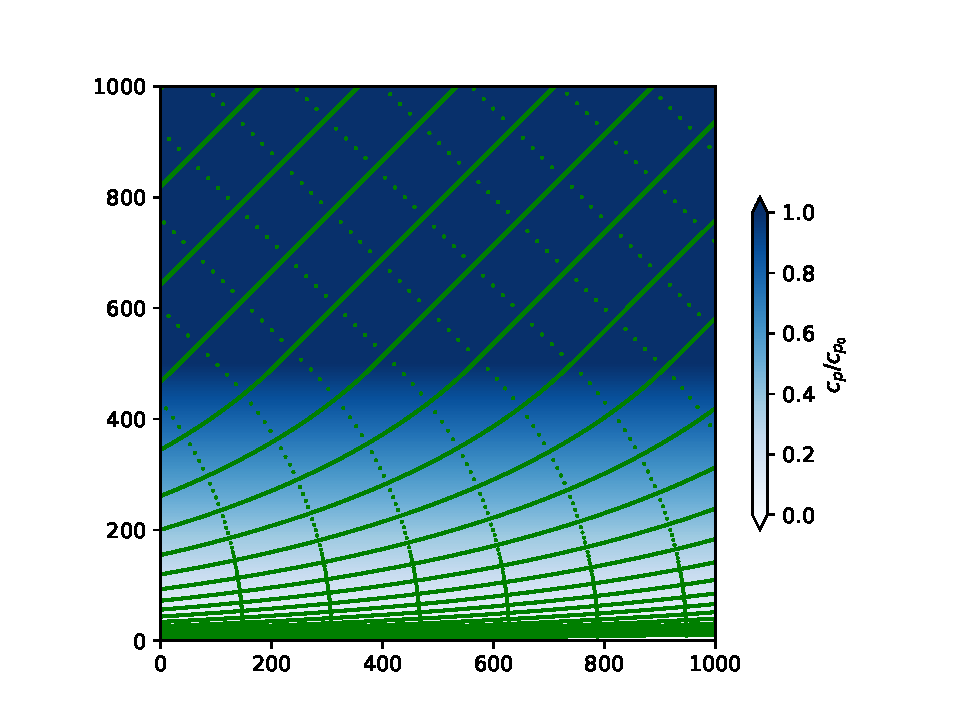
\includegraphics{figs/Waves/RaytraceStraight}
    \caption{Crests of waves moving into shallower water (as indicated by the blue colors). Initially parallel out at sea, the waves crests bend in towards the shoreline.  Dashed lines are wave ``rays'', and identify where  a certain point along the crest propagates to.  ``rays'' are perpendicular to the wave crests everyewhere. }
    \label{fig:RaytraceStraight}  
  \end{center}
\end{figure}


The refraction of waves explains why ``point breaks'' often have more stronger surf than ``beach breaks'' (\fref{fig:RaytraceHeadland}).  As waves are bent towards the headland there is a convergence of energy as rays become closer together that is added to the convergence of energy as the water gets shallower. Of course point breaks are also favoured by surfers because the wave that breaks at the point then progressively breaks as it moves on shore, lending for a longer ride into shore (\fref{fig:Rincon}).

\begin{figure}[hbt]
  \begin{center}
    \includegraphics{figs/Waves/Raytraceheadland}
    \caption{Crests of waves moving towards a headland.  Note the headland extends underwater (colors).  Note the concentration of rays at the wave-ward side of the headland.}
    \label{fig:RaytraceHeadland}  
  \end{center}
\end{figure}

\begin{figure}[hbt]
  \begin{center}
    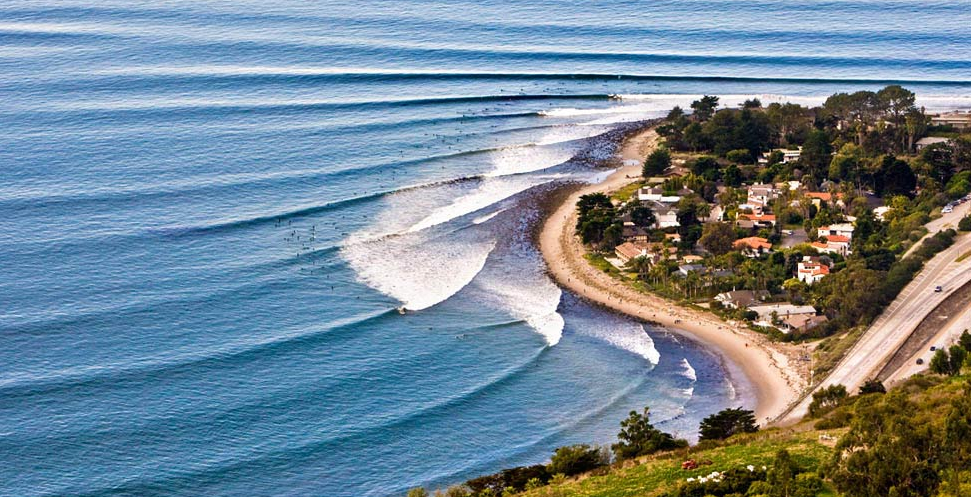
\includegraphics{figs/Waves/Rincon}
    \caption{Long period swell at Rincon (southern California), a classic point break.  }
    \label{fig:Rincon}  
  \end{center}
\end{figure}

Diffraction also leads to bent wavefronts, but is fundamentally due to cylindrical spreading of the wavefront.  We know that when we drop a pebble into a pool cylindrical waves will radiate from where the pebble hits the surface.  A related effect will occur on the lee side of a barrier like an island or a breakwater. The corner of the island is like a wave source for the calm water beyond, and the waves will spread out to fill the calm water in a cylindrical pattern (\fref{fig:WaveDiffraction}).  This will happen, even if the water is all one depth, so it is not due to refraction, though both phenomena can happen at the same time.    

\begin{figure}[hbt]
  \begin{center}
    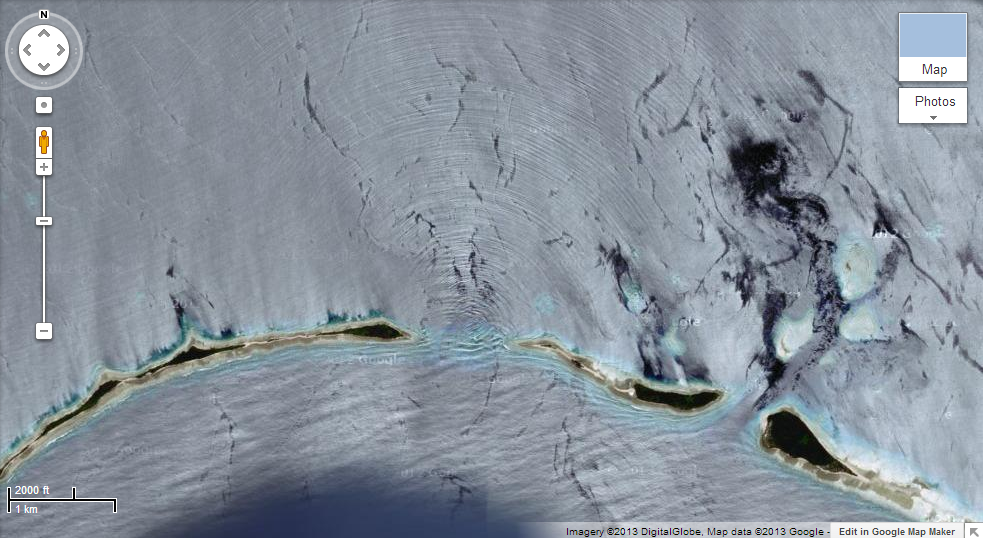
\includegraphics{figs/Waves/WaveDiffraction}
    \caption{Wave diffraction through a gap between two islands.  The swell is coming from the SSE and hits the gap from which radiates waves as approximate cylinders. \href{https://www.reddit.com/r/Physics/comments/1c5vd1/messing_about_on_google_maps_and_i_found_a_giant/}{From Reddit!} }
    \label{fig:WaveDiffraction}  
  \end{center}
\end{figure}
 
 

\section{Non-linearity}

The physics we have discussed so far applies to linear waves, i.e. waves for which the amplitude of the wave is much less than the water depth. If the wave amplitude becomes comparable to the water depth, the waves will become non-linear.  Usually non-linear waves require some sort of numerical simulation, but we can readily see how non-linear waves might steepen and break on a beach by considering the phase speed of the crest versus the through.

Normally, we consider the phase speed constant, however if the water depth changes drastically due to the, the water depth will be significantly larger at the crest $h_C$ than in the trough $h_T$ (\fref{fig:SketchNonLinearWave}).  This leads to steepening as the crest overtakes the trough, eventually leading to a vertical wave face and breaking.  

\begin{marginfigure}
    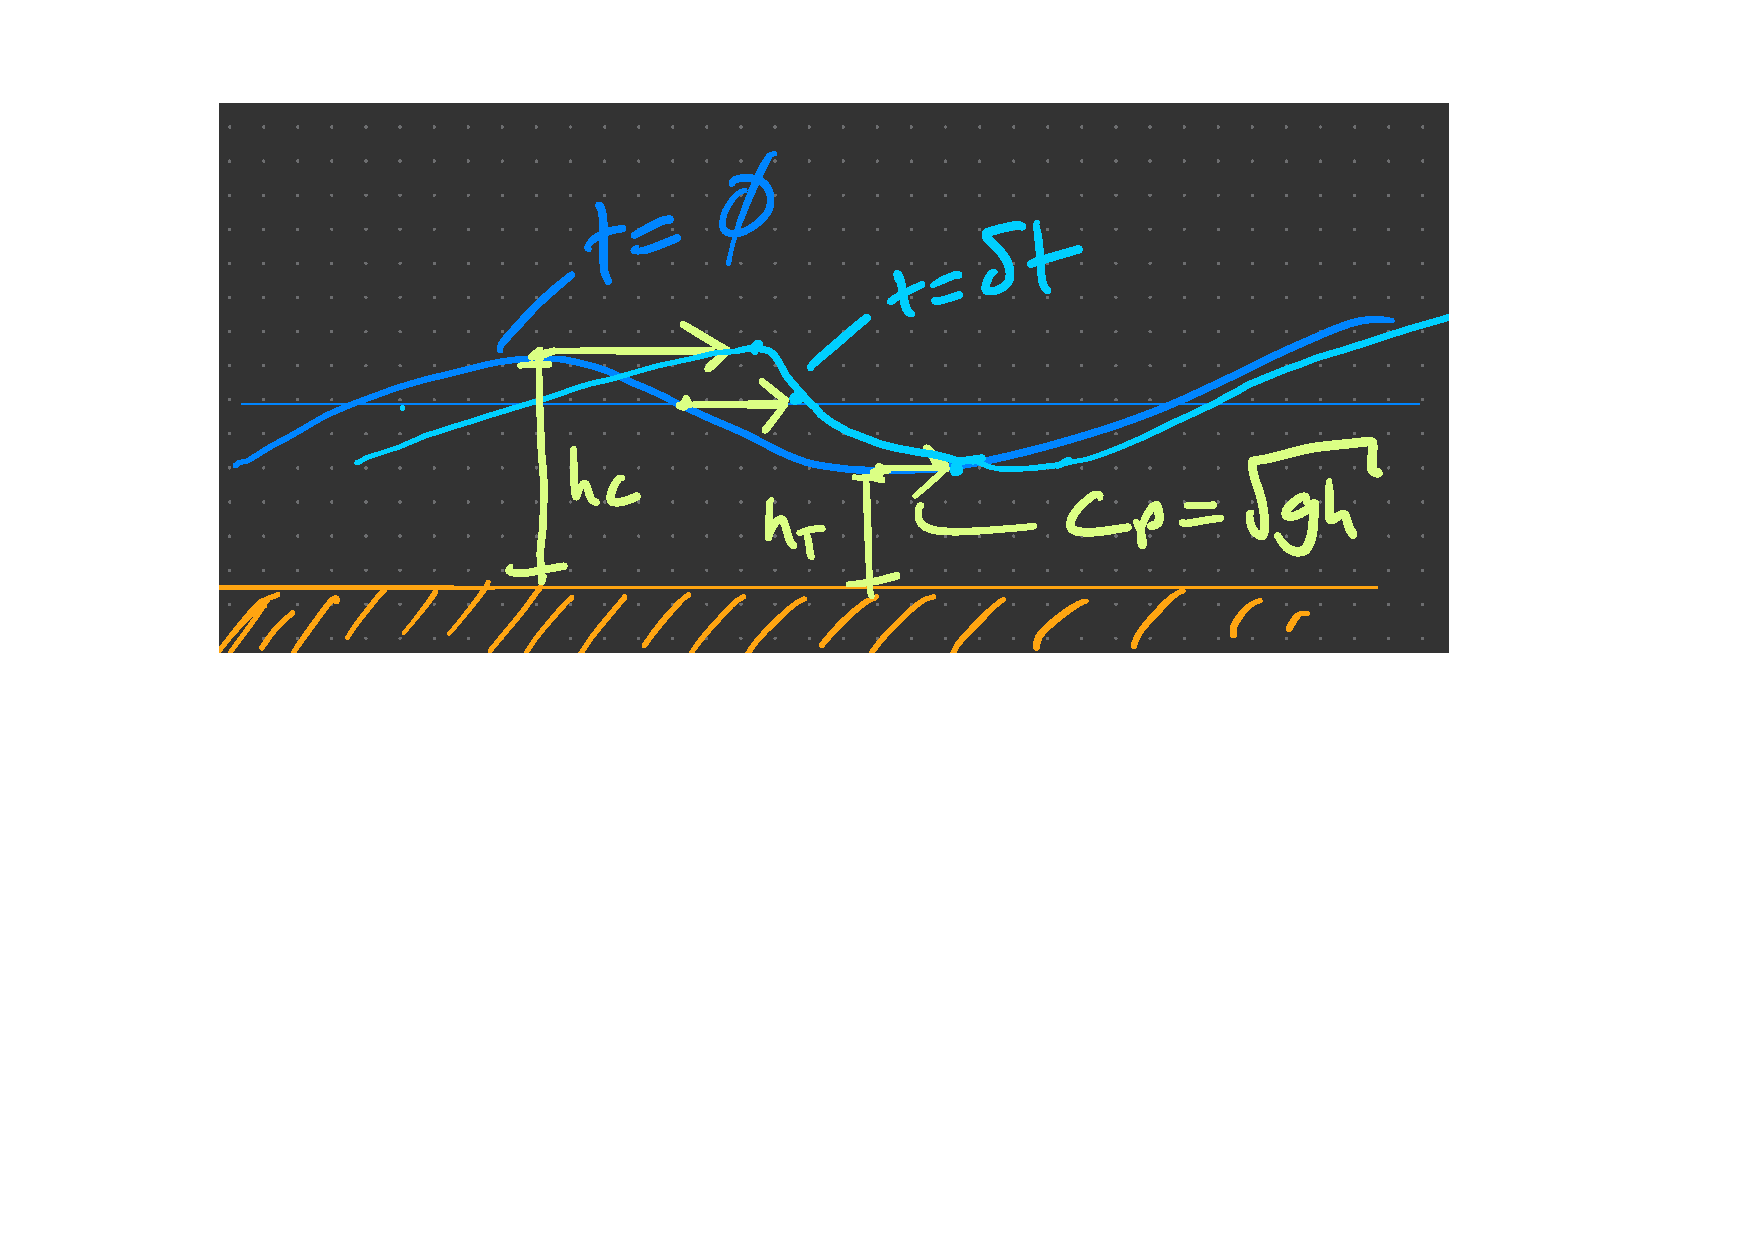
\includegraphics{figs/Waves/SketchNonLinearWave}
    \caption{Sketch of steepening wave at two different times.  The crest moves faster than the trough because the water depth is greater, and hence the wave steepens.}
    \label{fig:SketchNonLinearWave} 
\end{marginfigure}

There are other forms of non-linear behaviour, including when waves interact with one another, but this is the most straight forward and largely responsible for breaking waves and bores.  

%%% Local Variables:
%%% mode: latex
%%% TeX-master: t
%%% End:
